% %
% This file is encoded in utf-8
% This file is modified from
% 1. http://exciton.eo.yzu.edu.tw/~lab/latex/latex_note.html
%    (元智大學模版 陳念波老師)
% 2. http://code.google.com/p/ntuthesis/
%    (臺大碩士、博士論文的Latex模板)
%%
\documentclass[12pt,p a4paper]{class/ncku_class}

\usepackage{CJKutf8}  %%% ZZZ %%% macro for Chinese/Japanese/Korean processing
\usepackage{CJKnumb} %%% ZZZ %%% for Chinese numbering capability
\usepackage[nospace]{cite}  % for smart citation
\usepackage{geometry}  % for easy margin settings
\usepackage{class/ncku_style} % 自定義nckuee.sty // cbj
\usepackage{booktabs}
\usepackage{caption}
\usepackage{threeparttable}

% 插圖套件 graphicx
% 使用者工作流程是用 pdftex 還是 latex + dvipdfmx?
% 視情況而有不同的參數
% 這裡作自動判斷
% 參考自
% http://www.tex.ac.uk/cgi-bin/texfaq2html?label=ifpdf
%%\newcommand\mydvipdfmxflow{dvipdfmx}P
%%\newcommand\mypdftexflow{pdftex}P
%%\ifx\pdfoutput\undefined
%%  % not running pdftex
%%  \usepackage[dvipdfm]{graphicx}
%%  \newcommand\myworkflow{dvipdfmx}  % set the flag for hyperref
%%\else
%%  \ifx\pdfoutput\relax
%%    % not running pdftex
%%    \usepackage[dvipdfm]{graphicx}
%%    \newcommand\myworkflow{dvipdfmx}  % set the flag
%%  \else
%%    % running pdftex, with...
%%    \ifnum\pdfoutput>0
%%      % ... PDF output
%%      \usepackage[pdftex]{graphicx}
%%      \newcommand\myworkflow{pdftex}  % set the flag
%%    \else
%%      %...DVI output
%%      \usepackage[dvipdfm]{graphicx}
%%      \newcommand\myworkflow{dvipdfmx}  % set the flag
%%    \fi
%%  \fi
%%\fi
      \usepackage[pdftex]{graphicx}
      \newcommand\myworkflow{pdftex}  % set the flag

% 增強功能型頁楣 / 頁腳套件
\usepackage{fancyhdr}  % 借用此套件來擺放浮水印
% (佔用了 central header)
% 不需要浮水印的使用者仍可利用此套件,產生所需的 header, footer
%
% 啟動 fancy header/footer 套件
\pagestyle{fancy}
\fancyhead{}  % reset left, central, right header to empty
\fancyfoot[C]{\thepage} %中間 footer 擺放頁碼
\renewcommand{\headrulewidth}{0pt} % header 的直線; 0pt 則無線

% 如果不需要任何浮水印,則請把下列介於 >>> 與 <<< 之間
% 的文字行關掉 (行首加上百分號)
%% 浮水印 >>>
%
% this file is encoded in utf-8
% v2.0 (Apr. 5, 2009)
% 如果浮水印不是全篇需要,請把下列介於 >>> 與 <<<
% 的「全篇浮水印專用碼」關掉 (行首加百分號)
% 參考自 Keith Reckdahl 寫的 "Using Imported Graphics in LATEX2e" (epslatex.pdf) p.39
% 如果只有特定頁需要浮水印
% 則依該頁屬性使用下列之一的命令 
% 普通頁命令 \thispagestyle{WaterMarkPage}
% plain 頁命令 \thispagestyle{PlainWaterMarkPage}
% empty 頁命令 \thispagestyle{EmptyWaterMarkPage}


% 將重複使用的浮水印章
% 圖檔是 my_watermark.xxx
% 副檔名可以不加,可以是 latex 系統能處裡的任何格式:pdf, gif, png, jpg, eps, ...
% 某些圖檔格式在某些工作流程可能需要作前置處裡。
% 例如,pdflatex 無法直接處理 eps 檔
%  latex + dvipdfmx 無法直接處理 pdf, gif, png, jpg, 需要用 ebb 小工具程式
%  對圖檔產生 .bb 對應檔。
%
% 寬為 5.1 cm
\newsavebox{\mywatermark}
%\sbox{\mywatermark}{
\includegraphics[keepaspectratio,%
%width=5.1cm]{ncku_watermark}} % // ncku_watermark.jpg 浮水印 // cbj

\sbox{\mywatermark}{
\includegraphics{header/ncku_watermark.jpg}
} % // ncku_watermark.jpg 浮水印 // Hong-Je

% 將 central header 擺放浮水印的巨集指令
\newcommand{\PlaceWaterMark}{\fancyhead[C]{\setlength{\unitlength}{1in}%
\begin{picture}(0,0)%
%\put(-1,-6.2){\usebox{\mywatermark}}% 圖檔擺放的位置座標
\put(-1.35,-6.55){\usebox{\mywatermark}}% 圖檔擺放的位置座標
\end{picture}}%
}

\fancyhead{}  % reset left, central, right header to empty
%% 如果不需整篇論文都要浮水印
%% 則下面  >>> 與 <<< 之間的程式碼請關閉
%% >>> 全篇浮水印
\PlaceWaterMark  % 每一頁都有浮水印 (除了 plain、empty 頁以外)

% 重新定義 plain 頁面
% 每張 plain 頁面 (每一章的第一頁) 也加浮水印

\fancypagestyle{plain}{%
\fancyhead{}%
\PlaceWaterMark%
\fancyfoot{}%
\fancyfoot[C]{\thepage}
\renewcommand{\headrulewidth}{0pt}%
\renewcommand{\footrulewidth}{0pt}%
}
%% <<< 全篇浮水印

%% 如果只有一、兩頁需要有浮水印
%% 可以在該頁 (有頁碼) 使用 \thispagestyle{WaterMarkPage}
%% 此命令不影響原有的 header、footer
\fancypagestyle{WaterMarkPage}{%
\PlaceWaterMark%
}

%% 如果只有一、兩頁 plain 頁需要有浮水印 (如 摘要、自傳等)
%% 可以在該頁 (有頁碼) 使用 \thispagestyle{PlainWaterMarkPage}
%% 只有頁碼與浮水印,沒有其他的 header、footer
%% 等同於 plain page style + water mark
\fancypagestyle{PlainWaterMarkPage}{%
\fancyhead{}%
\PlaceWaterMark%
\fancyfoot{}%
\fancyfoot[C]{\thepage}
\renewcommand{\headrulewidth}{0pt}%
\renewcommand{\footrulewidth}{0pt}%
}

%% 如果只有一、兩頁 empty 頁需要有浮水印 (如封面、書名頁)
%% 可以在該頁 (無頁碼) 使用 \thispagestyle{EmptyWaterMarkPage}
%% 等同於 empty page style + water mark
\fancypagestyle{EmptyWaterMarkPage}{%
\fancyhead{}%
\PlaceWaterMark%
\fancyfoot{}%
\renewcommand{\headrulewidth}{0pt}%
\renewcommand{\footrulewidth}{0pt}%
}

%% <<< 浮水印
% 如需額外的頁楣 (header) 或 footer,請在 header/header_footer.tex 裡依例修改
% 它的預設內容是都關掉,可依需要打開
%
% this file is encoded in utf-8
% v2.0 (Apr. 5, 2009)

%%%%%%% 其他的 header (left, right) 定義
% 底下定義了一些常見的 header 型式
% 預設情況是關掉的
% 使用者可以視需要將之打開
% 也就是把下列介於 >>> 與 <<< 之間
% 的文字行打開 (行首去掉百分號)

%% header >>>
%\renewcommand{\chaptermark}[1]{%
%\markboth{\prechaptername\ \thechapter\ \postchaptername%
%\ #1}{}%
%}  %定義 header 使用的「章」層級的戳記
%\fancyhead[L]{} % 左 header 為空
%\fancyhead[R]{\leftmark}  % 右 header 擺放「章」層級的戳記 (以 \leftmark 叫出)
%\renewcommand{\headrulewidth}{0.4pt}  % header 的直線 0.4pt; 0pt 則無線
%% <<< header

%%%%%%% 其他的 footer (left, right) 定義
% 底下定義了一些常見的 footer 型式
% 預設情況是關掉的
% 使用者可以視需要將之打開
% 也就是把下列介於 >>> 與 <<< 之間
% 的文字行打開 (行首去掉百分號)

%% footer >>>
%\fancyfoot[L]{} % 左 footer 為空
%\fancyfoot[R]{\small{YZU \LaTeX\ v2.0}} % 右 footer 擺放論文格式版本
%\renewcommand{\footrulewidth}{0.4 pt} % footer 的直線 0.4pt; 0pt 則無線
%% <<< footer


%%%%%%%%%%%%%%%%%%%%%%%%%%%%%%
%%%% 非必要的套件,但很實用
\usepackage{amsmath} % 各式 AMS 數學功能
\usepackage{amssymb} % 各式 AMS 數學符號
\usepackage{mathrsfs} %草寫體數學符號,在數學模式裡用 \mathscr{E} 得草寫 E
\usepackage{listings} % 程式列表套件

%%%%%%%%%%%%%%
% // 可自行增加所需套件 // cbj
%\usepackage{subfig}
%%%%%%%%%%%%%%
\usepackage{subfigure}
\usepackage{graphicx} \graphicspath{{images/}}
\usepackage{psfrag} % text replacement in figure
\usepackage{amsmath}
\usepackage{bm}
\usepackage{mathtools}
\usepackage{hyperref}
\hypersetup{
colorlinks,%
citecolor=blue,%
filecolor=blue,%
linkcolor=blue,%
urlcolor=blue%
}
%%\usepackage{url}
%\usepackage{rotating} % table rotation
%\usepackage{amssymb}
\usepackage{array}
\usepackage{threeparttable} % table note
\usepackage{multirow} % newline on the tabular of a table.
%%%%%%%%%%%%%%
%---
\usepackage{tabularx}
\usepackage{url}
\usepackage[usenames,dvipsnames]{xcolor}
\usepackage{pgf}
\usepackage{tikz}
% \usetikzlibrary{arrows,automata,positioning}
\usetikzlibrary{arrows,shapes}
%
% listing setting
\lstset{
breaklines=true,% 過長的程式行可斷行
extendedchars=false,% 中文處理不需要 extendedchars
texcl=true,% 中文註解需要有 TeX 處理過的 comment line, 所以設成 true
comment=[l]\%\%,% 以雙「百分號」做為程式中文註解的起頭標記,配合 MATLAB
basicstyle=\small,% 小號字體, 約 10 pt 大小
commentstyle=\upshape,% 預設是斜體字,會影響註解裏的英文,改用正體
%language=Octave % 會將一些 octave 指令以粗體顯示
}

\usepackage{url} % 在文稿中引用網址,可以用 \url{http://www.yzu.edu.tw} 方式

%%%% 以上為非必要套件
%%%%%%%%%%%p%%%%%%%%%%%%%%%%%%%

%%% 以下是 hyperref 套件
%%%%%%%%%%%%%%%%%%%%%%%%%%%%%%
% hyperref 會擾亂 cite.sty 對文獻號碼縮編的排版,所以依據
% http://www.ctan.org/tex-archive/macros/latex/contrib/hyperref/
% 作如下的更動,使得 hyperref 不做文獻號碼的超連結。
\makeatletter
\def\NAT@parse{\typeout{This is a fake Natbib command to fool Hyperref.}}
\makeatother

% hyperlinkable table of contents
% 章節目錄、圖表超連結
%%\ifx\myworkflow\mydvipdfmxflow
%%	\usepackage[dvipdfmx, debug, colorlinks, linkcolor=black, citecolor=black, urlcolor=black, unicode]{hyperref}
%%\else
%%	\usepackage[pdftex, debug, colorlinks, linkcolor=black, citecolor=black, urlcolor=black, unicode]{hyperref}	
%%\fi
%自定義
\usepackage{hyperref}
\hypersetup{colorlinks, citecolor=blue,filecolor=blue,linkcolor=blue,urlcolor=blue}

% if hyperref is not used (e.g., in LyX application)
% define dummy \phantomsection for those occurences
%   in yzu_frontpages.tex, yzu_backpages.tex, my_appendix.tex
%%\ifx\hypersetup\undefined
%%	\newcommand\phantomsection{}
%%\fi
% hyperref跟algorithm衝突,hyperref必須放在algorithm前面
\usepackage{algorithm}
%\usepackage{algorithmic}
\usepackage{algpseudocode}
\usepackage{enumerate}
%\usepackage{subfig}
%%%% 以上為所有套件
%%%%
%%%%


%% global page layout
%\newcommand{\mybaselinestretch}{1.5}  %行距 1.5 倍 + 20%, (約為 double space)
%\renewcommand{\bapselinestrpetch}{\mybapselinestretch}  % 論文行距預設值
%\parskip=2ex  % 段落之間的間隔為兩個 x 的高度
%\parindent = 0Pt  % 段首內縮由 CJpK 控制,所以這裡就設成不內縮

%%%%%%%%%%%%%%%%%%%%%%%%%%%%%
%  end of preamble
%%%%%%%%%%%%%%%%%%%%%%%%%%%%%

%%%%%%%%%%%%%%%%%%%%%%%%%%%%%
%  Thesis Information // cbj (在frontpage資料夾內ncku_thesis_cover 設定)
%%%%%%%%%%%%%%%%%%%%%%%%%%%%%

%%\renewcommand{\enTitle}{An Edge Enhancement Algorithm for Upscaled Images}  % 英文標題
%%\renewcommand{\zhTitle}{針對放大後影像之邊緣增強演算法}  %中文標題
%%\renewcommand{\authorZhName}{陳宏哲}  %作者中文姓名
%%\renewcommand{\authorEnName}{Hong-Jhe Chen}  %作者英文姓名
%%%\renewcommand{\authorStudentID}{Q36991097}  %作者學號
%%\renewcommand{\advisorZhName}{戴顯權}  %指導教授中文姓名
%%\renewcommand{\advisorEnName}{Shen-Chuan Tai}  %指導教授英文姓名
%%\renewcommand{\zhUniv}{國立成功大學}
%%\renewcommand{\enUniv}{National Cheng Kung University}
%%%\renewcommand{\zhCollegeName}{電機資訊學院}  %學院中文名稱
%%%\renewcommand{\enCollegeName}{College of Electrical Enginnering and Computer Science}  % 學院英文名稱
%%\renewcommand{\zhDepartmentName}{電腦與通信工程研究所}  %系所中文名稱
%%\renewcommand{\enDepartmentName}{Institute of Computer and Communication Engineering Department of Electrical Engineering}  % 系所英文名稱
%%\renewcommand{\rocYear}{一〇一}  %中華民國紀年年份
%%\renewcommand{\zhMonth}{六}  %中文月份
%%\renewcommand{\enYear}{2012}  %公元紀年
%%\renewcommand{\enMonth}{June}  %英文月份
%%\renewcommand{\oralDate}{101 年 6 月 19 日}  %口試日期

%
\begin{document}
\begin{CJK}{UTF8}{bkai}   %%% ZZZ %%%  <<< 在這裡更改預設中文字型、編碼 // 設定標楷體字型 // cbj
% 編碼:UTF8, Bg5, ...
% 中文字型名稱:TeXLive 安裝有一套明體字 bsmi, 楷書與其他字型視你的 LaTeX CJK 系統裝設情況而定

% 針對 latex + dvipdfmx 工作流程在 hyperref 套件的影響下,圖檔的辨識力退化
% 所作的權宜措施。可能是因為 TeXLive2007 hyperref 裏的
% 客製 graphicx / dvipdfmx 的設定檔不夠新
\ifx\myworkflow\mydvipdfmxflow
	\DeclareGraphicsExtensions{.pdf,.png,.jpg,.eps}
	\DeclareGraphicsRule{.pdf}{eps}{.bb}{}
	\DeclareGraphicsRule{.png}{eps}{.bb}{}
	\DeclareGraphicsRule{.jpg}{eps}{.bb}{}
\fi

% global CJK setting
\CJKindent  %%% ZZZ %%%  段首內縮兩格

% 載入中文名詞的定義:例如,Figure -->「圖」, Chapter -->「第 x 章」
%
% this file is encoded in utf-8
% v2.0 (Apr. 5, 2009)

% 下列中文名詞的定義,如果以註解方式關閉取消,
% 則會以系統原先的預設值 (英文) 替代
% 名詞 \prechaptername 預設值為 Chapter
% 名詞 \postchaptername 預設值為空字串
% 名詞 \tablename 預設值為 Table
% 名詞 \figurename 預設值為 Figure
%\renewcommand\prechaptername{第} % 出現在每一章的開頭的「第 x 章」
%\renewcommand\postchaptername{章}
%\renewcommand{\tablename}{表} % 在文章中 table caption 會以「表 x」表示
%\renewcommand{\figurename}{圖} % 在文章中 figure caption 會以「圖 x」表示

% 下列中文名詞的定義,用於論文固定的各部分之命名 (出現於目錄與該頁標題)
\newcommand{\nameInnerCover}{書名頁}
\newcommand{\nameCommitteeForm}{論文口試委員審定書}
\newcommand{\nameCopyrightForm}{授權書}
\newcommand{\nameCabstract}{中文摘要}
\newcommand{\nameEabstract}{Abstract} %大寫用於內文
\newcommand{\nameEabstractc}{Abstract} %小寫用於目錄c
\newcommand{\nameAckn}{ACKNOWLEDGEMENTS}
\newcommand{\nameAcknc}{Acknowledgements}
\newcommand{\nameToc}{CONTENTS}
\newcommand{\nameTocc}{Contents}
\newcommand{\nameLot}{LIST OF TABLES}
\newcommand{\nameLotc}{List of Tables}
\newcommand{\nameTof}{LIST OF FIGURES}
\newcommand{\nameTofc}{List of Figures}
\newcommand{\nameSlist}{LIST OF SYMBOLS}
\newcommand{\nameSlistc}{List of Symbols}
\newcommand{\nameVita}{VITA}
\newcommand{\nameVitac}{Vita}
 % 主標題名稱定義 // 摘要 (Abstract), ... 等 // cbj

% 如果不需要以中文數字一、二、三呈現章別,例如「第一章」
% 則請把下列介於 >>> 與 <<< 之間
% 的文字行關掉 (行首加上百分號), 會以「第 1 章」呈現
%% 中文數字章別 >>>
%\input{yzu_chnum.tex}
%% <<< 中文數字章別

%%% 以下是載入前頁、本文、後頁
%====================
%  Front Pages // cbj
%  1. 封面頁 2. 口委中英文簽名單 3. 誌謝 4. 中英文摘要
%  5. 論文目錄 6. 圖表目錄 7. 符號說明
%  1&2定義於nckuee.sty ; 3&4&7放置在資料夾 frontpages\目錄下)
%====================
%% // nckuee.sty 定義 // cbj

% 產生論文封面
\nckuEEtitlepage
% 產生口試委員會簽名單
%\nckuEEoralpage
% 產生口試委員簽名單(en)
% \nckuEEenoralpage

%\newpage
%\setcounter{page}{1}
%\pagenumbering{roman}

%%%%%%%%%%%%%%%%%%%%%%%%%%%%%%%
%       封面內頁
%%%%%%%%%%%%%%%%%%%%%%%%%%%%%%%
% % unmark to add inner cover
%\newpage
%\thispagestyle{empty}
%\thispagestyle{EmptyWaterMarkPage}
%\nckuEEtitlepage


%%%%%%%%%%%%%%%%%%%%%%%%%%%%%%%
%       中文摘要
%%%%%%%%%%%%%%%%%%%%%%%%%%%%%%%

% 可以利用如下自定義的command (定義在nckuee.sty)
% ======
%\begin{zhAbstract}  %中文摘要
%現今許多先進的測量方法已被開發來觀測組蛋白修飾的確切位置,但是這些方法針對每種細胞株上測量不同的組蛋白修飾是件非常耗時且昂貴的實驗,為了解決這個困境,在近期的研究中,已有許多方法透過基因序列來預測各種組蛋白修飾,然而基因序列是無法提供細胞株特異性的資訊,導致在預測不同細胞株的組蛋白修飾時會遭遇很大的瓶頸,因此本研究引入了基因序列以及甲基化數據,並且利用卷積神經網路來改善預測不同細胞株的組蛋白修飾。

本研究將"啟動模塊"的特殊架構加入卷積神經網路中,以此來同時抓取不同序列長度的特徵。接著,我們利用"分層批次"的學習演算法,有效地在不平衡的資料集中訓練模型。最後,我們將混和的基因序列及甲基化數據基於上述的方法進行訓練,並從中萃取出具有細胞株特異性資訊的特徵向量來預測組蛋白修飾。

在實驗中,結果顯示我們設計的模型超越了基線模型,尤其是在最不平衡的類別上得到最明顯的改善。此外,我們也對不同輸入數據對效能的影響進行分析,結果表明結合基因序列及甲基化數據進行訓練的模型,相較於單獨只使用一種數據訓練的模型,不管在哪一種組蛋白修飾上都有顯著的提升。最後,我們進一步利用視覺化工具發現我們設計的模型的確能學習到細胞株特異性的資訊。

綜合以上的結果及分析,我們證實了利用改良的卷積神經網路並且結合基因序列及甲基化數據是有助於預測不同細胞株的組蛋白變異。
% 我們分別利用基因序列及甲基化的數據進行訓練及特徵萃取,並且進一步的混合這兩者的數據進行預測

% 人類基因組錯綜複雜的調控一直是遺傳學上關注的議題之一,許多生物學家利用調控區域上的變化進行觀察及分析,來破譯各種不同的基因調控機制及疾病。組蛋白就是調控基因的成員之一,它能透過自身的修飾來改變染色質的特性,在表觀遺傳上啟到致關重要的作用,因此有許多先進的測量方法已被開發來觀測組蛋白修飾的確切位置,然而這些方法要針對不同的細胞株測量各種組蛋白修飾是件非常耗時且昂貴的實驗,為了解決這個困境,現有的方法利用大量公開的資料集對未測量或是丟失的資料進行預測,以幫助後續更完整的分析。

% 因此為了加強對不同細胞株的預測,本研究加入了具有細胞株甲基化數據並且結合基因序列來預測組蛋白修飾確切的結合位點。

% 這是因為人類所有細胞株中的基因序列都是相同的,以至於無法提供任何有關細胞特異性的資訊,

% 在發表過的研究中,已有許多方法成功地利用基因序列來預測各種組蛋白修飾,並且得到不錯的成績,然而單純只使用基因序列來預測不同細胞株的組蛋白修飾會遭遇到很大的瓶頸,因此本研究引入了具有細胞株特異性的甲基化及基因序列的數據,並且透過新穎的卷積神經網路架構來改善預測組蛋白修飾的結合位點。

% 但是同時要對不同細胞株的染色質預測時,單純只使用基因序列的資料,這是因為人類所有細胞的基因序列都是相同的,然而染色質會因為細胞株的特異性有所不同。

% 因此本研究提出了基於深度學習的方法從基因序列及甲基化的資料中萃取特徵,來預測組蛋白修飾確切的結合位點

% DNA + DL --> methylation --> 引出我們到底怎麼做的 --> 模型的改善 --> 結果及結論

\begin{flushleft}
\mbox{{\bf 關鍵字}:卷積神經網路、資料差補、組蛋白修飾、甲基化、細胞株特異性}
\end{flushleft}
 % // 可以引入front_cabstract.tex檔案或在此編輯 // cbj
%\end{zhAbstract}

% ...等
% ======

% 在此直接定義如下
%%%%%%%%%%%%%%%%
%
\newpage
% // HongJhe 頁碼起始
\setcounter{page}{1}
\pagenumbering{roman}
% create an entry in table of contents for 中文摘要
\phantomsection % for hyperref to register this
\addcontentsline{toc}{chapter}{\nameCabstract}
% aligned to the center of the page
\begin{center}
% font size (relative to 12 pt):
% \large (14pt) < \Large (18pt) < \LARGE (20pt) < \huge (24pt)< \Huge (24 pt)
% Set the line spacing to single for the names (to compress the lines)
\renewcommand{\baselinestretch}{1}   %行距 1 倍
% it needs a font size changing command to be effective
\LARGE{\zhTitle}\\  %中文題目
\vspace{0.83cm}
% \makebox is a text box with specified width;
% option s: stretch
% use \makebox to make sure
% each text field occupies the same width
%\makebox[1.5cm][c]{\large{學生:}}
\hspace{0.5in}
\renewcommand{\thefootnote}{\fnsymbol{footnote}}
\makebox[3.5cm][l]{\large{\authorZhName\footnote[1]{}}}\footnotetext[1]{{學生}} % 學生中文姓名
%\hfill
%
%\makebox[3cm][c]{\large{指導教授:}}
\makebox[3.5cm][l]{\large{\advisorZhName\footnote[2]{}}}\footnotetext[2]{{指導教授}} \\ %指導教授中文姓名
%
\vspace{0.42cm}
%
\large{\zhUniv}\large{\zhDepartmentName}\\ %校名系所名
\vspace{0.83cm}
%\vfill
\makebox[2.7cm][c]{\large{摘要}}
\end{center}
% Resume the line spacing to the desired setting
\renewcommand{\baselinestretch}{\mybaselinestretch}   %恢復原設定
%it needs a font size changing command to be effective
% restore the font size to normal
\normalsize
%%%%%%%%%%%%%
\par  % 摘要首段空格 by SianJhe
現今許多先進的測量方法已被開發來觀測組蛋白修飾的確切位置,但是這些方法針對每種細胞株上測量不同的組蛋白修飾是件非常耗時且昂貴的實驗,為了解決這個困境,在近期的研究中,已有許多方法透過基因序列來預測各種組蛋白修飾,然而基因序列是無法提供細胞株特異性的資訊,導致在預測不同細胞株的組蛋白修飾時會遭遇很大的瓶頸,因此本研究引入了基因序列以及甲基化數據,並且利用卷積神經網路來改善預測不同細胞株的組蛋白修飾。

本研究將"啟動模塊"的特殊架構加入卷積神經網路中,以此來同時抓取不同序列長度的特徵。接著,我們利用"分層批次"的學習演算法,有效地在不平衡的資料集中訓練模型。最後,我們將混和的基因序列及甲基化數據基於上述的方法進行訓練,並從中萃取出具有細胞株特異性資訊的特徵向量來預測組蛋白修飾。

在實驗中,結果顯示我們設計的模型超越了基線模型,尤其是在最不平衡的類別上得到最明顯的改善。此外,我們也對不同輸入數據對效能的影響進行分析,結果表明結合基因序列及甲基化數據進行訓練的模型,相較於單獨只使用一種數據訓練的模型,不管在哪一種組蛋白修飾上都有顯著的提升。最後,我們進一步利用視覺化工具發現我們設計的模型的確能學習到細胞株特異性的資訊。

綜合以上的結果及分析,我們證實了利用改良的卷積神經網路並且結合基因序列及甲基化數據是有助於預測不同細胞株的組蛋白變異。
% 我們分別利用基因序列及甲基化的數據進行訓練及特徵萃取,並且進一步的混合這兩者的數據進行預測

% 人類基因組錯綜複雜的調控一直是遺傳學上關注的議題之一,許多生物學家利用調控區域上的變化進行觀察及分析,來破譯各種不同的基因調控機制及疾病。組蛋白就是調控基因的成員之一,它能透過自身的修飾來改變染色質的特性,在表觀遺傳上啟到致關重要的作用,因此有許多先進的測量方法已被開發來觀測組蛋白修飾的確切位置,然而這些方法要針對不同的細胞株測量各種組蛋白修飾是件非常耗時且昂貴的實驗,為了解決這個困境,現有的方法利用大量公開的資料集對未測量或是丟失的資料進行預測,以幫助後續更完整的分析。

% 因此為了加強對不同細胞株的預測,本研究加入了具有細胞株甲基化數據並且結合基因序列來預測組蛋白修飾確切的結合位點。

% 這是因為人類所有細胞株中的基因序列都是相同的,以至於無法提供任何有關細胞特異性的資訊,

% 在發表過的研究中,已有許多方法成功地利用基因序列來預測各種組蛋白修飾,並且得到不錯的成績,然而單純只使用基因序列來預測不同細胞株的組蛋白修飾會遭遇到很大的瓶頸,因此本研究引入了具有細胞株特異性的甲基化及基因序列的數據,並且透過新穎的卷積神經網路架構來改善預測組蛋白修飾的結合位點。

% 但是同時要對不同細胞株的染色質預測時,單純只使用基因序列的資料,這是因為人類所有細胞的基因序列都是相同的,然而染色質會因為細胞株的特異性有所不同。

% 因此本研究提出了基於深度學習的方法從基因序列及甲基化的資料中萃取特徵,來預測組蛋白修飾確切的結合位點

% DNA + DL --> methylation --> 引出我們到底怎麼做的 --> 模型的改善 --> 結果及結論

\begin{flushleft}
\mbox{{\bf 關鍵字}:卷積神經網路、資料差補、組蛋白修飾、甲基化、細胞株特異性}
\end{flushleft}
 % // 可以引入front_eabstract.tex檔案或在此編輯 // cbj



%%%%%%%%%%%%%%%%%%%%%%%%%%%%%%%
%       英文摘要
%%%%%%%%%%%%%%%%%%%%%%%%%%%%%%%
%
%[method 1]

% 可以利用如下自定義的command (定義在nckuee.sty)
% ======
%\begin{enAbstract}  %英文摘要
%Nowadays, many advanced measurement methods have been developed to observe the exact binding of histone modifications. However, it is a very time-consuming and expensive experiment to measure different histone modifications on each cell line. In order to solve this dilemma, In recent researches, there have been many methods to predict various histone modifications through DNA sequences. However, DNA sequences cannot provide any cell line-specific information, which leads to a big bottleneck in predicting histone modifications in different cell lines. Therefore, this study introduced DNA sequences and methylation data, and utilized convolutional neural network to improve the prediction of histone modifications in different cell lines.

In this research, the special structure of the "inception module" is added to the convolutional neural network to capture features of different sequence lengths at the same time. Next, we use the "stratified mini-batch" mechanism to effectively train the model on the unbalanced dataset. We finally train the mixed DNA sequences and methylation data based on the above methods, and extract feature vectors with cell line-specific information to predict histone modifications.

In the experiment, the results showed that the model we designed outperforms the baseline model, especially in the most unbalanced class to get the most obvious improvement. Besides, we analyze the effects of different input data for performance. The experimental results show that the model trained with DNA sequence and methylation data has significantly better performance in any histone modification than amodel trained with only one type of data. Finally, we further used visualization tools to find out that the model we designed could indeed learn cell line-specific information.

Based on the above results and analysis, we confirmed that the use of an improved convolutional neural network combined with DNA sequence and methylation data is helpful for predicting histone variation in different cell lines.

\begin{flushleft}
{{\bf Keywords}: Convolutional Neural Network, Data Imputation, Histone Modification, DNA methylation, Specificity of Cell Line}
\end{flushleft}
 % // 可以引入front_eabstract.tex檔案或在此編輯 // cbj
%\end{enAbstract}

%[method 2]
\newpage
% create an entry in table of contents for 英文摘要
\phantomsection % for hyperref to register this
\addcontentsline{toc}{chapter}{\nameEabstract} % // HongJhe marked

% aligned to the center of the page
\begin{center}
% font size:
% \large (14pt) < \Large (18pt) < \LARGE (20pt) < \huge (24pt)< \Huge (24 pt)
% Set the line spacing to single for the names (to compress the lines)
\renewcommand{\baselinestretch}{1}   %行距 1 倍
%\large % it needs a font size changing command to be effective
\LARGE{\enTitle}\\  %英文題目
\vspace{0.83cm}
% \makebox is a text box with specified width;
% option s: stretch
% use \makebox to make sure
% each text field occupies the same width
%\makebox[2cm][s]{\large{Student: }}
\hspace{0.45in}
\renewcommand{\thefootnote}{\fnsymbol{footnote}}
\makebox[5cm][l]{\large{\authorEnName\footnote[1]{}}}\footnotetext[1]{{Student}} % 學生英文姓名
%\hfill
%
%\makebox[2cm][s]{\large{Advisor: }}
\makebox[5cm][l]{\large{\advisorEnName\footnote[2]{}}}\footnotetext[2]{{Advisor}} \\ %教授英文姓名
%
\vspace{0.42cm}
\large{\enDepartmentName}\\ %英文系所全名
%
\large{\enUniv}\\  %英文校名
\vspace{0.83cm}
%\vfill
%
\large{\nameEabstractc}\\
%\vspace{0.5cm}
\end{center}

% Resume the line spacing the desired setting
\renewcommand{\baselinestretch}{\mybaselinestretch}   %恢復原設定
%\large %it needs a font size changing command to be effective
% restore the font size to normal
\normalsize
%%%%%%%%%%%%%
Nowadays, many advanced measurement methods have been developed to observe the exact binding of histone modifications. However, it is a very time-consuming and expensive experiment to measure different histone modifications on each cell line. In order to solve this dilemma, In recent researches, there have been many methods to predict various histone modifications through DNA sequences. However, DNA sequences cannot provide any cell line-specific information, which leads to a big bottleneck in predicting histone modifications in different cell lines. Therefore, this study introduced DNA sequences and methylation data, and utilized convolutional neural network to improve the prediction of histone modifications in different cell lines.

In this research, the special structure of the "inception module" is added to the convolutional neural network to capture features of different sequence lengths at the same time. Next, we use the "stratified mini-batch" mechanism to effectively train the model on the unbalanced dataset. We finally train the mixed DNA sequences and methylation data based on the above methods, and extract feature vectors with cell line-specific information to predict histone modifications.

In the experiment, the results showed that the model we designed outperforms the baseline model, especially in the most unbalanced class to get the most obvious improvement. Besides, we analyze the effects of different input data for performance. The experimental results show that the model trained with DNA sequence and methylation data has significantly better performance in any histone modification than amodel trained with only one type of data. Finally, we further used visualization tools to find out that the model we designed could indeed learn cell line-specific information.

Based on the above results and analysis, we confirmed that the use of an improved convolutional neural network combined with DNA sequence and methylation data is helpful for predicting histone variation in different cell lines.

\begin{flushleft}
{{\bf Keywords}: Convolutional Neural Network, Data Imputation, Histone Modification, DNA methylation, Specificity of Cell Line}
\end{flushleft}
 % // 可以引入front_eabstract.tex檔案或在此編輯 // cbj


%%%%%%%%%%%%%%%%%%%%%%%%%%%%%%%
%       誌謝
%%%%%%%%%%%%%%%%%%%%%%%%%%%%%%%
%
% Acknowledgment
% ================================
% \newpage
% \phantomsection % for hyperref to register this
% %\addcontentsline{toc}{chapter}{\nameAcknc}

% \begin{zhAckn}  %誌謝
% Add your acknowledgements here.

\begin{flushright}
\mbox{Syu-Min Cyu}
\end{flushright} % // 可以引入front_ackn.tex檔案或在此編輯 // cbj
% \end{zhAckn}
% ================================

%\chapter*{\nameAckn} %\makebox{} is fragile; need protect
%Add your acknowledgements here.

\begin{flushright}
\mbox{Syu-Min Cyu}
\end{flushright} % // 可以引入my_ackn.tex檔案或在此編輯 // cbj
%%testjsjtoejiojsoijtoijos

%%%%%%%%%%%%%%%%%%%%%%%%%%%%%%%
%       目錄
%%%%%%%%%%%%%%%%%%%%%%%%%%%%%%%
%
% Table of contents
\newpage
\renewcommand{\contentsname}{\nameToc}
%\makebox{} is fragile; need protect
\phantomsection % for hyperref to register this
\addcontentsline{toc}{chapter}{\nameTocc}
\tableofcontents

%%%%%%%%%%%%%%%%%%%%%%%%%%%%%%%
%       表目錄
%%%%%%%%%%%%%%%%%%%%%%%%%%%%%%%
%
% List of Tables
\newpage
\renewcommand{\listtablename}{\nameLot}
%\makebox{} is fragile; need protect
\phantomsection % for hyperref to register this
\addcontentsline{toc}{chapter}{\nameLotc}
\listoftables

%%%%%%%%%%%%%%%%%%%%%%%%%%%%%%%
%       圖目錄
%%%%%%%%%%%%%%%%%%%%%%%%%%%%%%%
%
% List of Figures
\newpage
\renewcommand{\listfigurename}{\nameTof}
%\makebox{} is fragile; need protect
\phantomsection % for hyperref to register this
\addcontentsline{toc}{chapter}{\nameTofc}
\listoffigures
%%%%%%%%%%%%%%%%%%%%%%%%%%%%%%%
%       符號說明
%%%%%%%%%%%%%%%%%%%%%%%%%%%%%%%
%
% Symbol list
% define new environment, based on standard description environment
% adapted from p.60~64, <<The LaTeX Companion>>, 1994, ISBN 0-201-54199-8

%\newcommand{\SymEntryLabel}[1]%
%  {\makebox[3cm][l]{#1}}
%%
%\newenvironment{SymEntry}
%   {\begin{list}{}%
%       {\renewcommand{\makelabel}{\SymEntryLabel}%
%        \setlength{\labelwidth}{3cm}%
%        \setlength{\leftmargin}{\labelwidth}%
%        }%
%   }%
%   {\end{list}}
%%%
%\newpage
%\chapter*{\nameSlist} %\makebox{} is fragile; need protect
%\phantomsection % for hyperref to register this
%\addcontentsline{toc}{chapter}{\nameSlistc}
%%
% this file is encoded in utf-8
% v2.0 (Apr. 5, 2009)
%  各符號以 \item[] 包住,然後接著寫說明
% 如果符號是數學符號,應以數學模式$$表示,以取得正確的字體
% 如果符號本身帶有方括號,則此符號可以用大括號 {} 包住保護
\begin{SymEntry}

\item[OLED]
Organic Light Emitting Diode

\item[$E$]
energy

\item[$e$]
the absolute value of the electron charge, $1.60\times10^{-19}\,\text{C}$
 
\item[$\mathscr{E}$]
electric field strength (V/cm)

\item[{$A[i,j]$}]
the  element of the matrix $A$ at $i$-th row, $j$-th column\\
矩陣 $A$ 的第 $i$ 列,第 $j$ 行的元素

\end{SymEntry}

\newpage
\setcounter{page}{1}
\pagenumbering{arabic}

%====================
%  Main Pages // cbj
%====================
% 本文
%\usepackage{geometry}  % for easy margin settings
%% margins setting // NCKU內頁設定 // cbj
%\geometry{verbose,a4paper,tmargin=2.3cm,bmargin=3.5cm,lmargin=2.5cm,rmargin=3cm}


\chapter{Introduction} \label{ch:1-introduction}
	\hspace{24pt}
% \renewcommand{\baselinestretch}{1.5}

\section{Background}
The bodies of humans and other complex animals are composed of trillions of cells.  Those cells can be classified into a large number (hundreds at least) of cell types which look and behavior radically different from each other (e.g.\ information processing neurons, insulin secreting $\beta$-cells, protective skin cells, etc.).  These cells are specialized to do particular tasks and the retain their identify during cell division; for example when a skin cell divides the outcome is two skin cells.  Interestingly, the basic nucleotide sequence of the genomes of these diverse cell types is essentially the same.  How then can these cell types be distinct?  The answer is thought to largely lie in differences in so called ``epigenetic marks'', namely DNA methylation and various histone modifications.

\subsection{DNA Methylation}
DNA methylation refers to the covalent addition of a methyl group to DNA nucleotides.
In vertebrates the primary form of DNA methylation is the addition of a methyl group to the C5 carbon residue of cytosines (fig.~\ref{f2}).  The reaction is catalyzed by DNA methyltransferases which act on cytosines found in CpG dinucleotides.  Some DNA methyltranferases function to maintain the methylation state of CpG's during cell division, ensuring that both daughter cells end up with methylated cytosines in the same places.  DNA methylation is heavily studied for two reasons.  First, DNA methylation can be measured more precisely and accurately than other epigenetic marks (via bisulfite sequence~\cite{frommer1992bisulfite}) and it is highly stable (DNA methylation is still largely intact after storage at 4$^{\circ}$C for 20 years ~\cite{li2018stability}).  Second, DNA methylation is known to be involved in several key biological processes, including regulation of gene expression, cell differentiation, and so on \cite{krueger2012dna}.

\begin{figure}[ht]
    \centering
    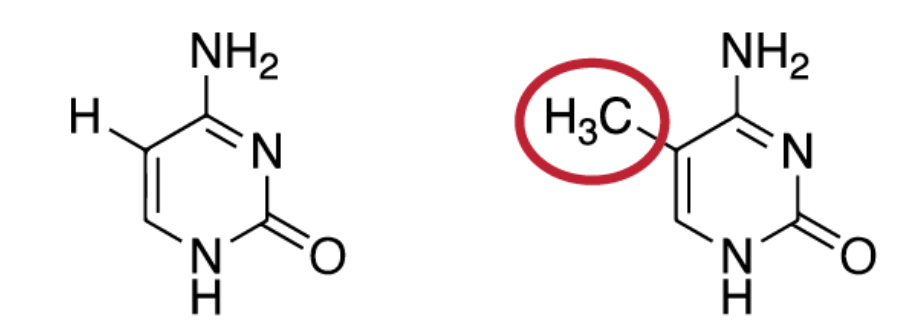
\includegraphics[width=0.8\columnwidth]{body/figure/figure2.png}
    \captionsetup{labelfont=bf}
    \renewcommand{\baselinestretch}{1.0}
    \caption[An illustration of DNA methylation]{The chemical structure of methylated (right) and unmethylated cytosine (left) is shown. (figure reproduced from \cite{enwiki:1028802025})}
    \label{f2}
\end{figure}


\subsection{Histone Modification}
Histones are a kind of structural DNA-binding protein that pack and order the DNA of eukaryotic chromosomes into basic structural units, called nucleosomes. A nucleosome consists of a segment of DNA, roughly 147 base pairs, wound around eight histone proteins. These are two copies of the four core histones (H2A, H2B, H3, H4) which form the structure, known as a histone octamer. Meanwhile, the H1 histone acts as the linker histone to stabilize inter-nucleosomal DNA but is not a one of core histones in the octamer.

\begin{figure}[H]
    \centering
    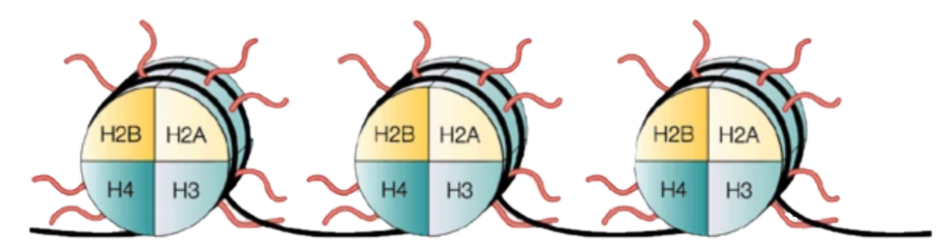
\includegraphics[width=1\columnwidth]{body/figure/figure1.png}
    \captionsetup{labelfont=bf}
    \renewcommand{\baselinestretch}{1.0}
    \caption[Structure of nucleosome]{The black curve is double-stranded DNA chain. It wraps around the eight core histones, and composes a spherical structure called a nucleosome. The red line is amino N-terminal tail, is major the part of occurring modification. (figure from \cite{marks2001histone})}
    \label{f1}
\end{figure}

Histone modification refers to covalent post-translational modification to histone amino N-terminal tail, including methylation, acetylation, phosphorylation and so on. Among these, the most common modifications are the methylation of arginine or lysine, and the acetylation of lysine. Histone modification affects a variety of biological processes, such as transcriptional activation and inactivation \cite{luger1997crystal}, as well as chromosome packaging \cite{peterson2004histones}, by altering structure \cite{allfrey1964acetylation} or recruiting histone modifier. Additionally, histone modifications are also helpful to identify some gene-regulatory regions. In Table\ref{t1}, it shows the five core histone marks and one histone acetylation mark, proposed by Roadmap Epigenomics Consortium \cite{kundaje2015integrative}, that are highly associated with different regulatory regions. According to these literatures, histone modifications play vital role in epigenetic research and provide useful information for further analysis.

\begin{table}[H]
    \centering
    \begin{tabular}{lc}
        \hline
        Histone modification    & Regulatory region \\\hline
        H3 lysine 4 monomethylation (H3K4me1) & Enhancer regions \\
        H3 lysine 4 trimethylation (H3K4me3)   & Promoter regions \\
        H3 lysine 9 trimethylation (H3K9me3) & Heterochromatin regions \\
        H3 lysine 27 acetylation (H3K27ac) & Enhancer regions \\
        H3 lysine 27 trimethylation (H3K27me3) & Polycomb repression \\
        H3 lysine 36 trimethylation (H3K36me3) & Transcribed regions \\\hline
    \end{tabular}
    \captionsetup{labelfont=bf}
    \caption{Table of histone modifications corresponding to regulatory regions}
    \label{t1}
\end{table}


\section{Problem Description}
In order to better understanding of epigenetic mechanism, quantitative detection of histone modification is important. Histone modifications are mainly profiled by chromatin-immunoprecipitation followed by sequencing (ChIP-seq). This method uses corresponding antibody for histone modifications or specific DNA-binding proteins to identify enriched loci within genome \cite{nakato2020methods}. The major advantage of ChIP-seq is the higher resolution and lower noise over chromatin immunoprecipitation with DNA microarray (ChIP-chip) \cite{massie2012mapping}. But, the disadvantage of ChIP-seq is still expensive and time-consuming, because it requires lots of tissues, so that profiling rare biological samples, such as primary cells and clinical samples, is constrained \cite{gilfillan2012limitations}. In this case, these biosamples may be rejected low-quality data resulting in the missing value, or identified lower quality data. It will cause bias in further analysis. Thus, data imputation methods are often used appropriately in this scenario.

Data imputation with computational methods attempt to utilize relation among different kinds of biological data to remove noise or reconstruct missing value. Currently, multiple public datasets are available to download. They are provided by the project conducted international collaboration of research groups, such as Encyclopedia of DNA Elements (ENCODE) project \cite{davis2018encyclopedia} and Roadmap Epigenomics project \cite{kundaje2015integrative}. These lots of available data is good for data imputation with computational method. Especially, machine-learning based or deep-learning based methods are data-driven approaches that are good at dealing with large amount of data. Thus, diverse bioinformatics studies in recent massively apply deep-learning methods, and expect a variety of frameworks of deep learning to discovery more insight in biological domain.

The most popular frameworks, convolutional neural network (CNN) and recurrent neural network (RNN), are extensively used to extract features. These are individually great at modeling translation invariant features by CNN, and modeling long-range interactions by RNN. According the properties of frameworks and biological data, we can choose the most appropriate model to fit on diverse tasks. For example, DeepBind uses CNN to predict binding site of DNA and RNA binding proteins by extracting features from DNA sequences, and allows to learn the correct motifs by different kernels in CNN \cite{alipanahi2015predicting}. Quang and Xue proposed new hybrid framework, called DanQ, that combines CNN and bi-directional long-short term memory(BiLSTM) network, which is a variant of RNN. It takes advantages of these frameworks to predict the functions of DNA sequences \cite{quang2016danq}. Min et al. proposed a deep learning framework, called DeepEnhancer, to classify enhancer regions from genomic sequences \cite{min2016deepenhancer}. The success of these methods shows that deep learning is a powerful tool for genomic researches. However, DNA sequences in different cell lines are identical. Above successful methods only extract features from DNA sequences, so that these methods are lack of power of making predictions in cell line-specific cases \cite{yin2019deephistone}\cite{chen2021deepcape}.

\section{Motivation}
Therefore, to overcome this limitation, there are many deep-learning based methods integrating DNA sequences and various biological experimental data. For example, Laiyi Fu et al. proposed a hybrid deep learning model additionally adding features from MeDIP-seq data and information of histone modification to predict DNA methylated states \cite{fu2019predicting}. Chen et al. proposed DeepCAPE, a deep CNN to predict enhancers via the combination of DNA sequences and DNase-seq data \cite{chen2021deepcape}. These papers in cell line-specific manner improve performance of data imputation for epigenetic data.

Besides, DNA methylation and histone modification not only individually supply useful insight in analysis but also have special interaction between themselves. Recent evidence indicates that DNA methylation and histone modification pathways can be interdependent, and this crosstalk can be mediated by biochemical interaction. For example, histone modification can directly help to DNA methylation, and DNA methylation might serve as a template for some histone modifications \cite{cedar2009linking}. As such, it is rational to integrate DNA sequences and DNA methylation information for the study of cell line-specific histone modifications.

\section{Objective}
In our research, we aim to find out whether introducing information from DNA methylation can help to improve prediction of binding sites of histone modifications. Motivated by the above understanding, we design deep-learning based approach to capture features from DNA sequences, while taking advantage of the relationship between histone modifications and DNA methylation signal. In order to ensure whether our hypothesis is effective, we use comprehensive experiments to validate our approach.


\chapter{Related Works} \label{ch:2-background}
	\hspace{24pt}
% \renewcommand{\baselinestretch}{1.5}

In this section we review previous studies that employ deep-learning based methods and integrate DNA sequences and various biological experimental data to predict histone modification.

Over the past decade, there are many studies of data imputation for epigenetic data that have applied deep-learning based methods. Zhou and Troyanskaya designed a model to observe the effect of non-coding variants, called DeepSEA. Although the main goal of their paper is not data imputation for histone modifications, they utilize CNN to extract regulatory sequence code from genomic sequence by learning to simultaneously predict large-scale chromatin-profiling data, including transcription factor, chromatin accessibility and histone modification, and use this model to analyze \cite{zhou2015predicting}. Quang and Xue proposed a new hybrid framework model, called DanQ, to solve the same task as DeepSEA and improve predictions. In the DanQ model, the convolution layers extract short-term information (regulatory motifs) from DNA sequences while the recurrent layers capture long-term dependencies between the regulatory motifs \cite{quang2016danq}. These methods select suitable architecture of model and take advantage of multi-task joint learning of various chromatin factors that share predictive features, and obtain satisfactory performance. But, these methods only focus on genomic features so that limits prediction of cell line-specific cases, because DNA sequences in any cell line are the same.

In order to overcome this limitation, these following methods introduce various biological experimental data, which is extracted by models to learn more cell line-specific information. Yin et al.\ designed CNNs to separately extract features from sequence information and chromatin accessibility data, and use joint module to combine features generated by CNNs. This model, called DeepHistone, not only accurate predicts the binding site of histone modifications, but learns correct motifs in each cell line by different convolutional layers \cite{yin2019deephistone}. Baisya and Lonardi developed a model, called DeepPTM, to predict the binding sites of histone modifications from DNA sequences and transcription factor binding data, combined with an effective pre-processing step in which they employ neighborhood cleaning rule to remove noisy training data. And, they report more accurate prediction from transcription factor binding data than from chromatin accessibility data \cite{baisya2020prediction}. These papers both select the biological experimental data highly related to gene expression. Lanchabtin and Qi further introduced 3D structure data of DNA interaction for better representation of DNA, due to 3D organization of chromatin in the cell have effects on regulatory regions, like promoter and enhancer. The model, called ChromeGCN, first extracts local genomic features from DNA sequences by convolutional layers, and then profile long-range 3D genomic information from organization of chromatin by graph convolutional layers \cite{lanchantin2020graph}.  Together, these studies indicate that deep-learning based method is able to extract patterns from biological domain and indeed improve performance by introducing other biological experimental data.

However, from view of data, above biological experimental data introduced is not general enough. Chromatin accessibility introduced by DeepHistone might not account for the entire genome \cite{yan2016genome}. Although this situation is not apparent in current advanced measurement technologies, chromatin accessibility data actually has lower coverage over whole genome than DNA methylation data, shown in Table~\ref{t2}. 3D organization of chromatin, Hi-C data, introduced by ChromeGCN have relatively low resolution in most available datasets, such as 25kb or 40kb \cite{zhang2018enhancing}.  This resolution is insufficient for histone modification prediction. There are various kinds of transcription factors which are considered by DeepPTM. But, many for many transcription factors binding data in most cell lines are not available on ENCODE website. As a result, DeepPTM is individually trained on same deep-learning framework against different cell lines, and generates models corresponding to cell lines. For instance, one is that using 30 transcription factors of H1, a kind of cell line, to predict 4 histone modifications, and another is that using 45 transcription factors of K562 to predict 3 histone modifications.

\begin{table}[H]%加入table環境指令以控制表格的位置、編號與標題,[h]代表將表格置於here,其他位置的標示請參考手冊
    \centering
    \begin{tabular}{lcc}
        \hline
        Cell line &  DNA methylation & Chromatin accessibility \\\hline
        A549 & 43582049 & 27235575 \\
        GM12878 & 38461546 & 10309402 \\
        K562 & 26944982 & 21450010 \\\hline
    \end{tabular}
    \renewcommand{\baselinestretch}{1.0}
    \captionsetup{labelfont=bf}
    \caption[Amount of active signals of coverage in whole genome]{Amount of active signals of coverage in whole genome. These cell lines are selected in this study to analyze}
    \label{t2}
\end{table}

In terms of model design, although DeepPTM has solved the problem of data generalization, it loses the advantages of multi-task model, such as data efficiency, reduced overfitting through shared representations, and fast learning by leveraging auxiliary information \cite{crawshaw2020multi}. Additionally, in most of the above mentioned methods implemented by CNN, the kernel size is fixed in each convolutional layer. In DeepSEA, kernel size of all convolution layers is set as eight \cite{zhou2015predicting}. In DnaQ, kernel size of a convolutional layer on top of RNN is set as twenty-six \cite{quang2016danq}. In DeepHistone, kernel size of all convolutional layers is set as nine \cite{yin2019deephistone}. In ChromeGCN, kernel size of all convolutional layers on top of graph convolutional layer is set as eight \cite{lanchantin2020graph}. Nevertheless, recent researches on CNN indicate that extracting features from the same input with different kernel sizes, called “inception module” by Szegedy et al., can improve performance \cite{szegedy2015going}\cite{tan2019mixconv}. This framework is not only good for image data but sequential data, including DNA sequences. Published bioinformatics methods have been shown apparent improvement by successfully introducing inception module into model. For instance, Zhang et al.\ designed a inception-like network with gating mechanism to concurrently capturing multiple local patterns and long-term association in DNA sequences, to predict nucleosome position \cite{zhang2018lenup}.


\chapter{Material and Method} \label{ch:3-proposed}
	\hspace{24pt}
% \renewcommand{\baselinestretch}{1.5}

This paper attempts to improve prediction of cell line-specific cases by utilizing DNA methylation signal, and introduce an inception module into the CNN to increase the ability to extract features. In our problem formulation, we define prediction of six histone modifications in a window as a binary classification task, given a fixed-length segment of DNA sequence and methylation signal. This is known as a multi-label classification task, where multiple labels can be positive at once.

\begin{figure}[H]
    \centering
    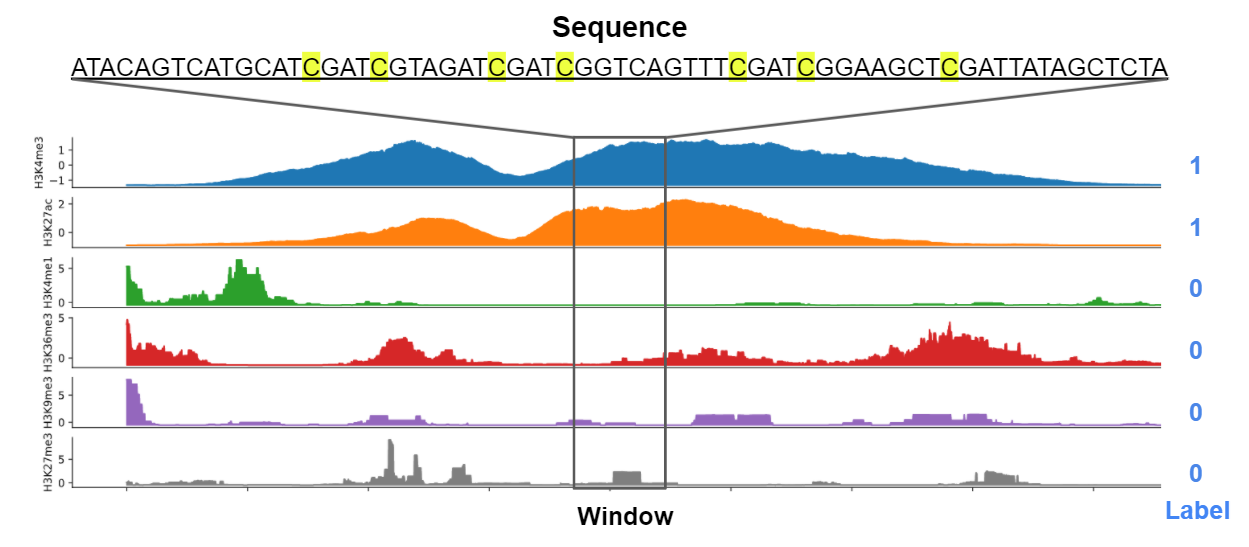
\includegraphics[width=1\columnwidth]{body/figure/figure3.png}
    \captionsetup{labelfont=bf}
    \renewcommand{\baselinestretch}{1.0}
    \caption[Pair of input and label]{The methylated cytosines are marked by yellow in DNA sequence.}
    \label{f3}
\end{figure}

\section{Data Preprocessing}
We download peak files of six histone modifications for three human epigenomes from the ENCODE project. These six histone modifications, including H3K4me1, H3K4me3, H3K9me3, H3K27ac, H3K27me3 and H3K36me3, are important markers that have been verified to be associated with specific functional regions in the genome, as shown in Table~\ref{t1}. For convenience and efficient experiment, we first select 3 epigenomes in the category of cell lines, which have complete dataset that six histone modifications and methylation signal. There are including A549, GM12878 and K562, where GM12878 and K562 are widely used in ENCODE and Roadmap project \cite{davis2018encyclopedia}\cite{kundaje2015integrative}.

Peak file is generated by peak calling algorithm, which is a step of standard pipeline of capturing protein-binding regions. This file indicates where is binding regions, called peak, in genome, and the signal value of binding regions. Given six peak files of each cell lines, we use a window of 200bp to scan the whole human genome with step 200 bp, and regard a window that has at least 100 bp overlap with peak as a histone modification binding site, shown in Figure~\ref{f3}. Our setting is similar to DeepHistone \cite{yin2019deephistone}, but we add additional rule that at least one positive peak in window. Because most of peaks of any histone modifications in genome is not active and not interesting to us, we add this rule to remove lots of windows, whose all labels are negative.

\begin{table}[H]%加入table環境指令以控制表格的位置、編號與標題,[h]代表將表格置於here,其他位置的標示請參考手冊
    \centering
    \begin{tabular}{lcccc}
    \hline
        Cell line & A549 & M12878 & K562	 \\\hline
        H3K4me3 & 163727 (0.06) & 253760 (0.32) & 154500 (0.1) \\
        H3K27ac & 697041 (0.23) & 294976 (0.37) & 227165 (0.14) \\
        H3K4me1 & 537240 (0.18) & 355490 (0.44) & 520504 (0.34) \\
        H3K36me3 & 1068720 (0.36) & 140428 (0.17) & 129438 (0.08) \\
        H3K9me3 & 223102 (0.08) & 63791 (0.08) & 51017 (0.03) \\
        H3K27me3 & 1000516 (0.34) & 63640 (0.08) & 745326 (0.49) \\\hline
        Total & 2961825 & 805361 & 1521904\\\hline
    \end{tabular}
    \captionsetup{labelfont=bf}
    \renewcommand{\baselinestretch}{1.0}
    \caption[Amount of windows of each cell line]{These entries are amount of positive peak of six histone modification in each cell line. The bottom row represents total number of windows.The number in the parenthesis is percentage of positive peak in each histone modification.}
    \label{t3}
\end{table}

We then download the human reference genome (GRCh38) and extract the 2000bp DNA sequence surrounding the center of each window as an input, since the motif for a special signal is may not be contained in the 1000bp \cite{lanchantin2020graph}, whereas DeepSEA, DanQ and DeepHistone set 1000bp. Next, we covert base of DNA sequence to value, and combine methylation signal into input matrix. These are separately encoded by one-hot encoding scheme, as well as positive-stranded and negative-stranded methylation percentage. As a result, the input of model is a 5 * 2000 matrix, including features from four bases and methylation.

After creating the pair of input features and label, we first divide each dataset of each cell line into ten partitions because whole dataset can not be stored in memory. To obtain more representative partition of dataset, we use stratified sampling to split against labels so that each partition of dataset has same distribution.

\section{Convolutional neural network on sequence data}
Convolutional neural network (CNN) is one of the most popular algorithms in deep-learning field. CNN has been successfully applied on many applications. Especially, it makes a lot of progress in image recognition, because shared weights and local connections in the CNN are employed to make full use of 2D input-data structures \cite{alzubaidi2021review}.

CNN is mainly composed of convolutional layer, pooling layer and fully connected layer. First, convolutional layer is a group of convolutional filters, also called kernels. Each kernel scan input data to extract local features with convolutional operation, and generate output called feature map \cite{alzubaidi2021review}. According to above description, we can apparently observe the property of convolutional layer that modeling invariant features. This allows CNNs effectively learn correct “motifs” from DNA sequences, that the patterns is learned by kernel. The diagram of convolutional layer is shown on following Figure~\ref{f4}.

\begin{figure}[H]
    \centering
    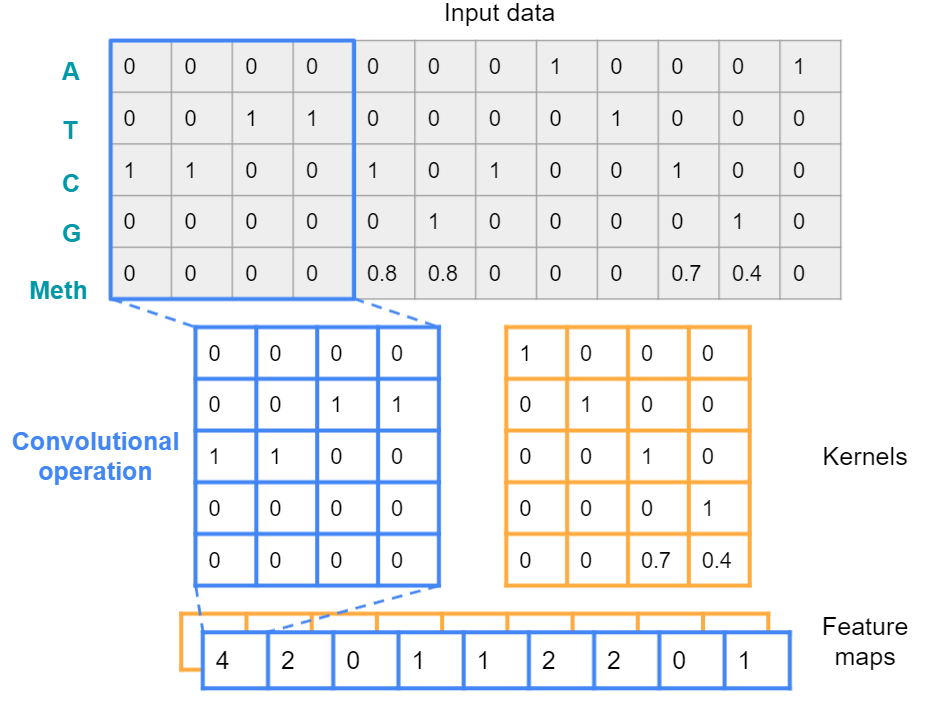
\includegraphics[width=1\columnwidth]{body/figure/figure4.png}
    \captionsetup{labelfont=bf}
    \renewcommand{\baselinestretch}{1.0}
    \caption[Convolutional operation]{Convolutional operation is that element-wised multiplication, and then summation. Parameters in kernels are like neuron in network, that is learned.}
    \label{f4}
\end{figure}

Second, pooling layer is that sampling the feature maps generated by convolutional layers. The main goal is to shrink feature maps, without lose important information. There are several types of pooling methods implemented in pooling layers, including max pooling, average pooling, and so on \cite{alzubaidi2021review}. The most common pooling layer is max pooling, shown in following Figure~\ref{f5}.

\begin{figure}[H]
    \centering
    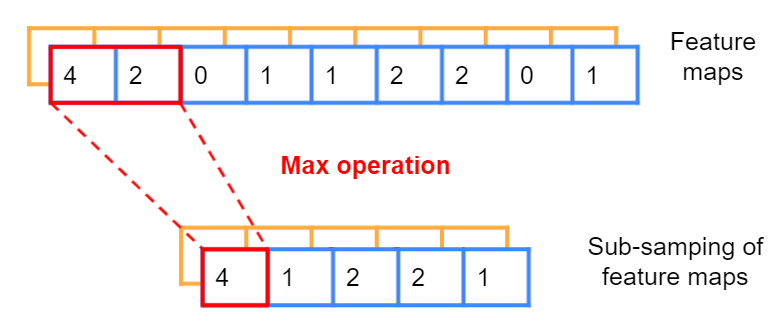
\includegraphics[width=0.9\columnwidth]{body/figure/figure5.png}
    \captionsetup{labelfont=bf}
    \renewcommand{\baselinestretch}{1.0}
    \caption[Operation of max pooling]{Pooling layer is similar to convolutional layer. It calculates within small region, also called kernel, and output one value in feature map.}
    \label{f5}
\end{figure}

Third, fully connected layer is often located on end of CNN and acts as classifier. Its input is the feature extracted by previous convolutional layers and pooling layers. Because input of fully connected layer is in the form of a vector, feature maps should be flatten as a vector \cite{alzubaidi2021review}. Then, the classifier takes feature vector to predict.

\begin{figure}[H]
    \centering
    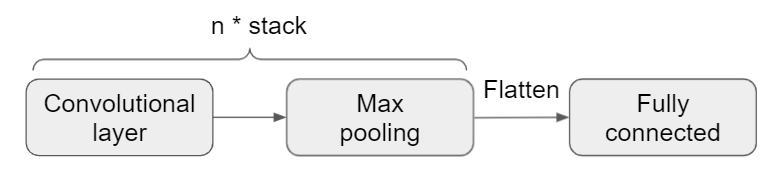
\includegraphics[width=0.9\columnwidth]{body/figure/figure6.png}
    \captionsetup{labelfont=bf}
    \renewcommand{\baselinestretch}{1.0}
    \caption[Standard pipeline of convolutional neural network]{Standard pipeline of convolutional neural network.}
    \label{f6}
\end{figure}

Figure~\ref{f6} is standard pipeline in CNN, which extracts features through convolutional layers and pooling layers, and then classifies through fully connected layers. Convolutional layers and pooling layers can be stacked many times to increase capability of CNN. Although there are many variants of CNN, main pipeline like Figure~\ref{f6} is not changed.

\section{Inception Module}
The trend in deep learning is that utilizing deeper and wider architectures to improve quality of networks. In 2014, Szegedy et al. introduce inception module into GoogLeNet. Inception module is designed by different kernel sizes to extract various scale features, shown in Figure~\ref{f7}. It makes model wider and gets better performance \cite{szegedy2015going}.

\begin{figure}[H]
    \centering
    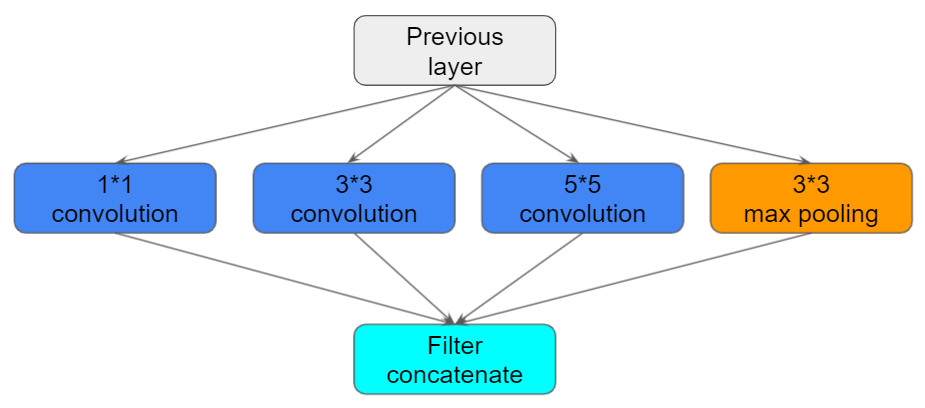
\includegraphics[width=0.8\columnwidth]{body/figure/figure7.png}
    \captionsetup{labelfont=bf}
    \renewcommand{\baselinestretch}{1.0}
    \caption[Naive version of inception module]{Naive version of inception module.}
    \label{f7}
\end{figure}

But, the complex model is readily to overfitting, and is not easily trained on limited computational source. This common problem has existed in model-based method for a long time. Accordingly, to overcome this problem, Szegedy et al. add two methods into model, 1 * 1 convolutional layer and global average pooling. First, 1 * 1 convolutional layer is just a convolutional layer whose kernel size is one. When it is added on top of convolutional layer, it can learn more non-linear information from previous layer, and effectively scale the dimensions of feature maps to reduce calculation in model, shown in Figure~\ref{f8} \cite{lin2013network}. Second, global average pooling is a kind of average pooling, whose kernel size is equal to size of feature map. This mechanism is located at the last pooling layer, to reduce parameters of connection between feature maps and fully connected layer \cite{lin2013network}. Hence, GoogLeNet is allowed for increasing the depth and width of the network, while keeping the computational budget constant. Also, GoogLeNet won the ImageNet Large-Scale Visual Recognition Challenge (ILSVRC) in 2014.

\begin{figure}[H]
    \centering
    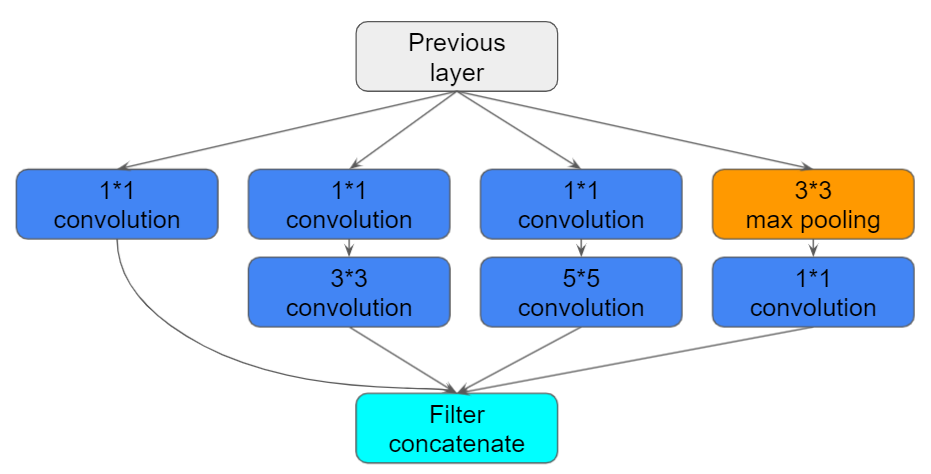
\includegraphics[width=0.8\columnwidth]{body/figure/figure8.png}
    \captionsetup{labelfont=bf}
    \renewcommand{\baselinestretch}{1.0}
    \caption[Final version of inception module]{Final version of inception module, implemented in GoogLeNet.}
    \label{f8}
\end{figure}

\section{Model Architecture} \label{method}
We select the convolutional neural network as our framework, which consists of multiple convolutional layers, pooling layers and fully connected layers, because convolutional layer is good at extracting motifs in genome. In addition, we add inception module into our model so that extract more representative features through kernels of different scales. The complete architecture is depicted in Figure~\ref{f12}, where detailed modules are used in Figure~\ref{f9}. The details of the structure are explained and summarized as follows:

\begin{figure}[H]
    \centering
    \subfigure[Input layer]{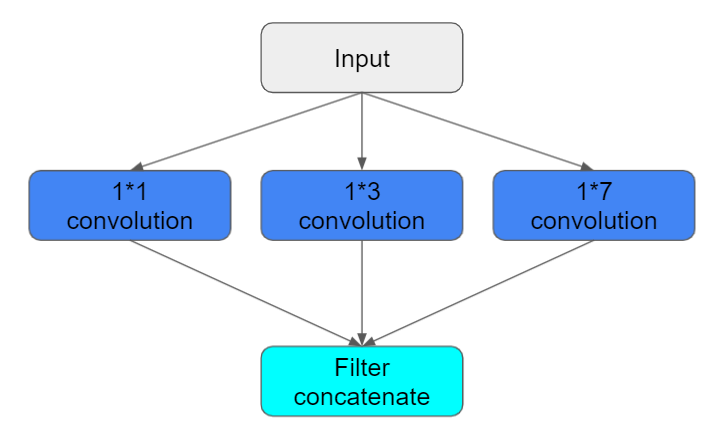
\includegraphics[width=0.65\columnwidth]{body/figure/figure9.png}}\\
    \centering
    \subfigure[Inception module-a]{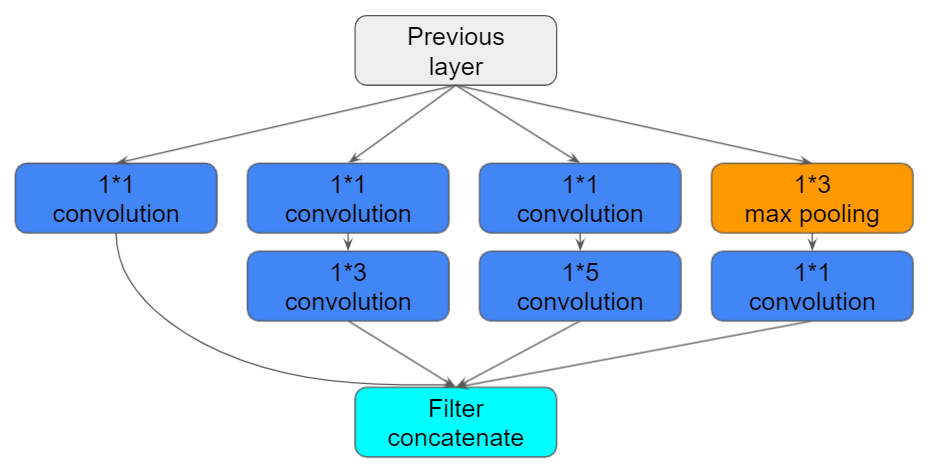
\includegraphics[width=0.75\columnwidth]{body/figure/figure10.png}}\\
    \centering
    \subfigure[Inception module-b]{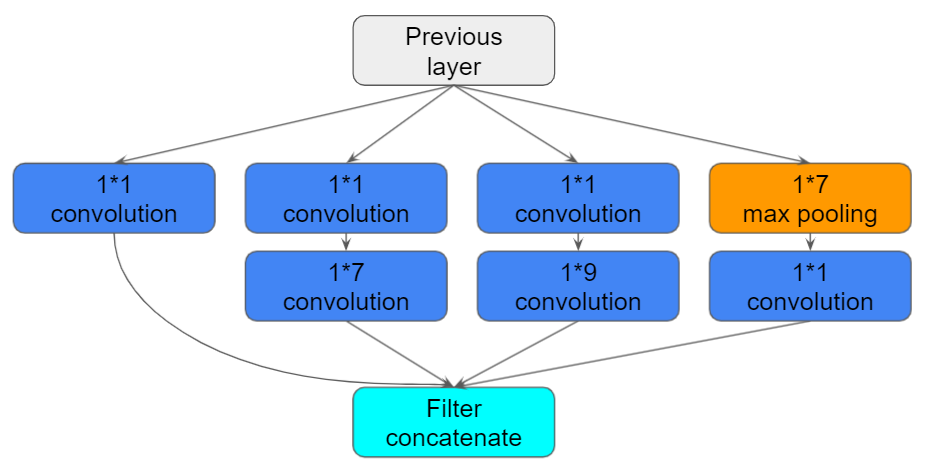
\includegraphics[width=0.75\columnwidth]{body/figure/figure11.png}}\\
    \captionsetup{labelfont=bf}
    \renewcommand{\baselinestretch}{1.0}
    \caption[Structure of detailed modules]{Inception module-b. 1 * n means that length n of sequence of extracting features at once.  The block of filter concatenate in all figures is to stack all feature maps from each branch together.}
    \label{f9}
\end{figure}

In terms of convolutional layer, we remove bias of all convolutional layers because of reducing parameters of model. It can not only avoid model too complex but increase batch size. Next, the outputs of all convolutional layers are orderly passed through the batch normalization layer and rectified linear unit (ReLU). They are respectively for avoiding overfitting and activation.

In terms of pooling layer, all max pooling layers of kernel size are three, and step with two. The goal of these layers is to sample the feature maps from previous layer, and reduce the length of feature map. After passing last pooling layer, one dropout layer with fifty percentage of dropped outputs was performed in training.

In terms of fully connected layers, they are located at the end of stacked convolutional layers and pooling layers, to predict histone modifications. We design two fully connected layers, individually 100 neurons and 6 neurons.

\begin{figure}[H]
    \centering
    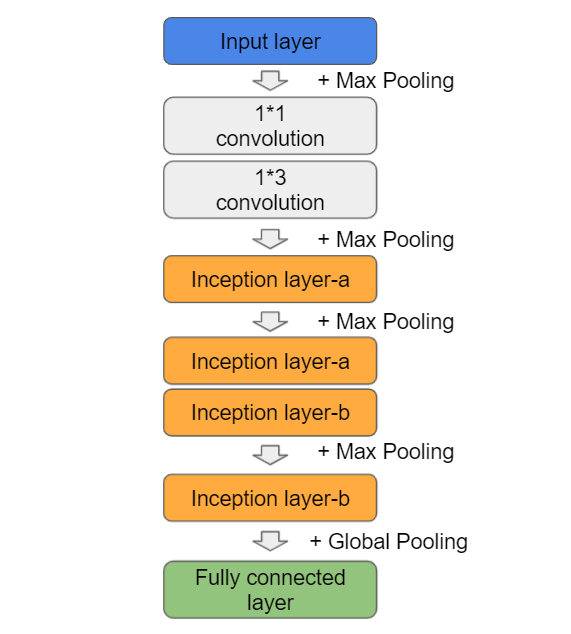
\includegraphics[width=0.7\columnwidth]{body/figure/figure12.png}
    \captionsetup{labelfont=bf}
    \renewcommand{\baselinestretch}{1.0}
    \caption[Complete architecture]{The overall architecture of our model. Global pooling represents global average pooling, located on top of the block of fully connected layer.}
    \label{f12}
\end{figure}

In terms of training methodology, our model is trained using stochastic gradient descent with momentum of 0.9, a learning rate of 0.01, and trained using a batch size of 300. For our loss function, we use the mean binary cross-entropy with sigmoid function \(\sigma\) across all labels $L$, shown in equation~\ref{eq:weight}.  In equation~\ref{eq:weight}, $w_\ell$ is the weight to scale the given to the loss of each positive element. It can deal with imbalance status in each class. According to Table~\ref{t3}, our dataset is imbalanced in class distribution. Hence, we set the weights inversely proportional to percentage of positive peaks for each histone modification, to mitigate the effects of this imbalance.

%%\[  F(y, \hat{y}) = \frac{1}{L}\sum_{l=1}^{L}-(w_l*y_i^llog\sigma(\hat{y}_i^l)+(1-y_i^l)log(1- \sigma(\hat{y}_i^l) ))\ \ (1)  \]

\begin{equation}
F(y, \hat{y}) = \frac{-1}{L}\sum_{\ell=1}^{L} \left( w_\ell\,y_i^\ell\log\sigma(\hat{y}_i^\ell) \,+\, (1-y_i^\ell)\log(1-\sigma \hat{y}_i^\ell) \right)
\label{eq:weight}
\end{equation}

\section{Stratified mini-batch}
However, only setting the weight in loss function is not enough to deal with imbalanced multi-label tasks, as shown in Section~\ref{strat}. Imbalanced learning is still a challenging issue because model-based methods for any task are significantly affected by skewed datasets \cite{buda2018systematic}. In order to obtain higher accuracy, the classifier tends to ignore labels with low frequency, which lead to more errors in minority classes. Therefore, Peng et al.\ propose the method, that introduce stratified sampling to modify the sampling operation of mini-batch learning, to solve this issue \cite{peng2021addressing}. In this paper, Peng et al.\ designed the two stratified sampling against label powerset and label. Label powerset-based stratification is that sampling dataset according to the distribution of all label combinations. But, this stratification select samples from a large number of labels combinations, resulting in the construction of a large mini-batch that is not suitable for the training of the model. Label-based stratification is that sampling dataset according to the distribution of all label classes. Compared to label powerset-based stratification, it only considers the number of label classes, that fewer number of stratifications is good for our limited computational resource. Accordingly, we introduce the label-based stratified sampling into mini-batch learning, to keep the distribution of each mini-batch the same as the whole dataset.

	
\chapter{Experiment and Result} \label{ch:4-simulation}
	\hspace{24pt}
\renewcommand{\baselinestretch}{1.5}

In this chapter, we will explain the detail of experiments. First, we describe the experimental environment in Section\ref{environment}. Second, we introduce the dataset from ENCODE, the method how to select within many datasets in Section\ref{dataset}. Third, before showing the performance, we early depict evaluation metrics in Section\ref{metric}. Fourth, we show experiment results from different models to compare their performance in Section\ref{performance}. Finally, we further analyze model by visualization of feature vectors in Section\ref{discuss}.

\section{Environment} \label{environment}
We use PyTorch, one of the most deep learning libraries \cite{paszke2017automatic}, to construct architecture of our model. And, the model designed by PyTorch can be trained and operated on a CUDA-capable Nvidia GPU to upgrade experimental efficiency. Our GPU is GEFORCE RTX 2070 SUPER. In order to more conveniently monitor model, we use Weights \& Biases (wandb) \cite{wandb} for logging hyperparameters and output metrics, then quickly visualize and compare results with dashboard on website.

\section{Dataset} \label{dataset}
We download datasets from the ENCODE project. This project is being conducted by ENCODE consortium, funded by the National Human Genome Research Institute. The goal of ENCODE is to build a comprehensive list of functional elements in the human genome. To high quality of analysis, ENCODE investigators employ a variety of assays and methods to identify various functional elements, and all generated data is available on ENOCDE website \cite{davis2018encyclopedia}.

We select three cell lines as datasets, including A549, GM12878 and K562. However, each epigenetic data on ENCODE website may be measured by different laboratories, while setting the different parameters in experiment that influence generated data. Hence, we select the dataset according to the warnings represented on ENCODE website. These warnings may indicate an error in the experimental metadata, or may indicate that the data itself does not meet some aspect of the consortium’s standards. There are three flag’s colors corresponding to the severity of the problem \cite{davis2018encyclopedia}.

\begin{figure}[H]
    \centering
    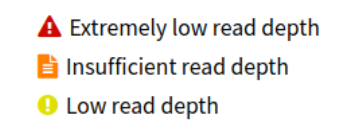
\includegraphics[width=0.5\columnwidth]{body/figure/figure13.png}
    \captionsetup{labelfont=bf}
    \renewcommand{\baselinestretch}{1.0}
    \caption[Example of warning levels]{This figure is screenshotted from ENCODE website. The example shows that different levels of severity in low read depth, which acts as metric to evaluate the quality of sequencing experiment.}
    \label{f13}
\end{figure}

Therefore, we choose datasets, that are less amount of warnings and lower level of warnings, to further analysis.

\section{Evaluation Metrics} \label{metric}
We use two metrics to evaluate our model. There are respectively area under the receiver operating characteristics curve (ROC) and area under the precision-recall curve (PRC). These metrics are common evaluations of a classifier’s prediction performance, which are threshold-free measures.

Before introducing area under ROC and area under PRC, we first introduce confusion matrix because these metrics are composed of the elements of this matrix. The confusion matrix consists of true positive (TP), false positive (FP), true negative (TN) and false negative (FN). shown in Figure~\ref{f14}. Each row of the matrix represents the instances in an actual class while each column represents the instances in a predicted class, or vice versa. The several basic metrics are calculated by elements of confusion matrix, including precision, recall (also called sensitivity) and specificity \cite{saito2015precision}, shown in function(2) ,(3) and (4).

\begin{figure}[H]
    \centering
    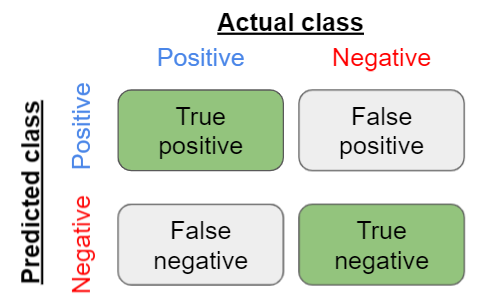
\includegraphics[width=0.65\columnwidth]{body/figure/figure14.png}
    \captionsetup{labelfont=bf}
    % \renewcommand{\baselinestretch}{1.0}
    \caption[Confusion matrix]{Confusion matrix.}
    \label{f14}
\end{figure}

\vspace{-1cm}
\[Precision : \frac{TP}{TP+FP}\ (2)\]
\[Recall(sensitivity) : \frac{TP}{TP+FN}\ (3),\ Specificity : \frac{TN}{TN+FP}\ (4)\]

Then, ROC is plotted by sensitivity and specificity. PRC is plotted by precision and recall. Areas under these curves are metrics that evaluating our model. In addition, these curves provide useful information of baseline (random classifier). The baseline showed in ROC is a diagonal line, whereas the baseline showed in PRC is dynamic. The baseline of PRC is determined by the ratio of positives (P) and negatives (N) as y = P / (P+N) \cite{saito2015precision}, shown in Figure~\ref{f15}.

\begin{figure}[H]
    \centering
    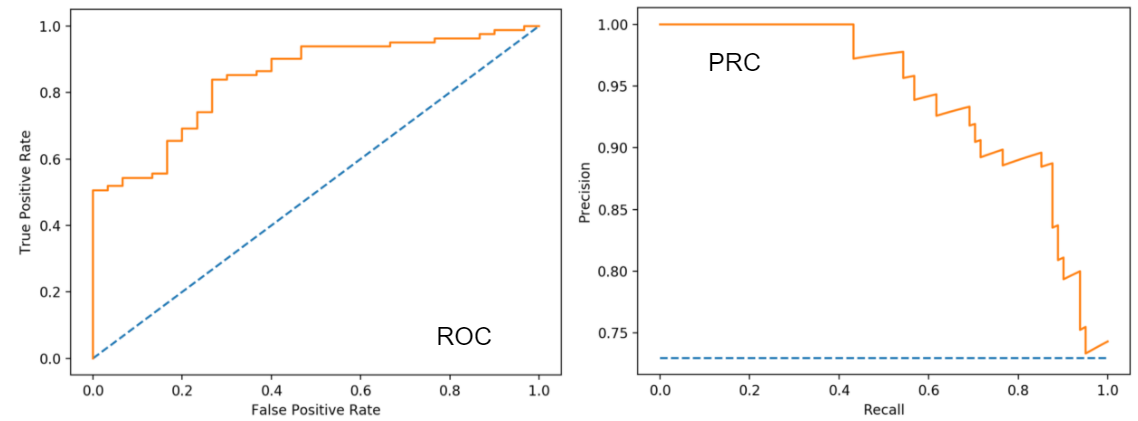
\includegraphics[width=1\columnwidth]{body/figure/figure15.png}
    \vspace{-1cm}
    \captionsetup{labelfont=bf}
    \renewcommand{\baselinestretch}{1.0}
    \caption[ROC and PRC]{Solid line represents monitored model. Dotted line represents baseline (random classifier). And, area under these curves represents performance of these models. (figure reproduced from \cite{rocprc})}
    \label{f15}
\end{figure}

\section{Prediction Performance} \label{performance}
In order to validate whether introducing techniques and features are helpful to our model. we design a series of following experiments to observe results. Finally, we will show the results of best model trained on all cell lines in Section\ref{cross}.

\subsection{Baseline}
We construct a CNN according to the architecture of DeepSEA \cite{zhou2015predicting}, which acts as baseline. The baseline is depicted in Figure~\ref{f16}, and is trained on same training methodology with our model, described in Section\ref{method}. Only difference is that amount of neurons in the last fully connected layer. We focus on data imputation of six histone modifications, instead of interaction of various chromatin states. Therefore, we change the amount of neurons in the last fully connected layer to six, that the number is amount of histone modifications we want to predict.

\begin{figure}[H]
    \centering
    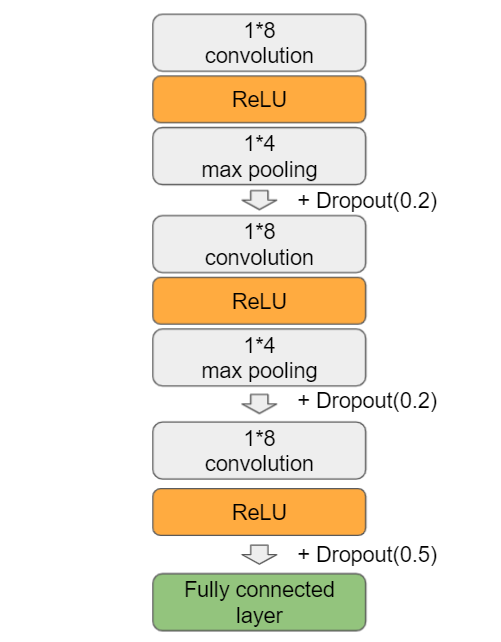
\includegraphics[width=0.6\columnwidth]{body/figure/figure16.png}
    \captionsetup{labelfont=bf}
    \renewcommand{\baselinestretch}{1.0}
    \caption[Framework of baseline]{The framework of baseline is same with DeepSEA.}
    \label{f16}
\end{figure}

\subsection{Inception Module}
To experimental efficiency, we first select nine partitions (1369713 windows) of K562 to train on baseline and our model, and then evaluate on one partition (152191 windows) of K562 to compare the results of these models. Accroding to Section\ref{metric}, we use area under ROC (AUROC) and area under PRC (AUPRC) as evaluation metrics.

Here, we want to observe the change of results after adding inception module into our model. Our model is named “Inception” in following tables. Apparently, we improve the prediction in all cases compared to baseline, shown in Table~\ref{t4} and Table~\ref{t5}.

\subsection{Stratified Mini-batch} \label{strat}
According to same settings with above experiment, we want to test whether stratified mini-batch is good for our task, that is imbalanced multi-label classification, shown in Table~\ref{t4} and Table~\ref{t5}. In the following tables, we use subscript to represent the model adding stratified mini-batch. In addition, we test on not only our model but also baseline, in order to check whether this mechanism only helps on special case.

\begin{table}[H]%加入table環境指令以控制表格的位置、編號與標題,[h]代表將表格置於here,其他位置的標示請參考手冊
    \centering
    \begin{tabular}{lcccc}
    \hline
    Model & Baseline & $Baseline_{stratified}$ & Inception & $Inception_{stratified}$ \\\hline
    H3K4me3 & 0.979 & 0.9819 & 0.9902 & \textbf{0.9927} \\
    H3K27ac & 0.9278 & 0.9334 & 0.9488 & \textbf{0.9549} \\
    H3K4me1 & 0.9672 & 0.9718 & 0.9745 & \textbf{0.9787} \\
    H3K36me3 & 0.985 & 0.9854 & 0.9857 & \textbf{0.9886} \\
    H3K9me3 & 0.9283 & 0.9429 & 0.9726 & \textbf{0.9762} \\
    H3K27me3 & 0.9923 & 0.9938 & 0.9964 & \textbf{0.9969} \\\hline
    \end{tabular}
    \captionsetup{labelfont=bf}
    \renewcommand{\baselinestretch}{1.0}
    \caption[Comparison of baseline and inception with AUROC]{This table represents performance with AUROC. Best predictive performance of each histone modification is shown in bold.}
    \label{t4}
\end{table}

\begin{table}[H]%加入table環境指令以控制表格的位置、編號與標題,[h]代表將表格置於here,其他位置的標示請參考手冊
    \centering
    \begin{tabular}{lcccc}
    \hline
    Model & Baseline & $Baseline_{stratified}$ & Inception & $Inception_{stratified}$ \\\hline
    H3K4me3 & 0.8995 & 0.9089 & 0.9365 & \textbf{0.9474} \\
    H3K27ac & 0.723 & 0.7385 & 0.7754 & \textbf{0.7934} \\
    H3K4me1 & 0.9388 & 0.9465 & 0.9501 & \textbf{0.9588} \\
    H3K36me3 & 0.8886 & 0.8905 & 0.9082 & \textbf{0.9208} \\
    H3K9me3 & 0.541 & 0.5911 & 0.7641 & \textbf{0.8114} \\
    H3K27me3 & 0.9905 & 0.9925 & 0.996 & \textbf{0.9965} \\\hline
    \end{tabular}
    \captionsetup{labelfont=bf}
    \renewcommand{\baselinestretch}{1.0}
    \caption[Comparison of baseline and inception with AUPRC]{This table represents performance with AUPRC. Best predictive performance of each histone modification is shown in bold.}
    \label{t5}
\end{table}

Regardless of the frameworks in above table, model adding this mechanism outperform original model. And, the model, which introduces inception module and stratified mini-batch into, gets the best results in above experiments. Hence, we decide to use this model to extract features from DNA sequences and DNA methylation signal, and then use these features to predict histone modifications.

\subsection{DNA methylation}
After confirming these techniques is helpful, we mainly want to observe how much different input features influence the results of model. We separately extract features from only DNA sequences, only DNA methylation signal and both, as well as represent them by subscript in following tables. It is same with above experiments that all models are trained on K562. In addition, we further check whether the framework of DeepSEA can also improve predition by adding features from DNA methylation signal, shown in Table~\ref{t6}, Table~\ref{t7}, Table~\ref{t8} and Table~\ref{t9}.

\begin{table}[H]%加入table環境指令以控制表格的位置、編號與標題,[h]代表將表格置於here,其他位置的標示請參考手冊
    \centering
    \begin{tabular}{lccc}
    \hline
    Model & $Baseline_{Meth}$ & $Baseline_{DNA}$ & $Baseline_{DNA+Meth}$ \\\hline
    H3K4me3 & 0.8963 & \underline{0.9741} & \textbf{0.9819} \\
    H3K27ac & 0.8475 & \underline{0.9172} & \textbf{0.9334} \\
    H3K4me1 & \underline{0.9435} & 0.8943 & \textbf{0.9718} \\
    H3K36me3 & \underline{0.9766} & 0.8982 & \textbf{0.9854} \\
    H3K9me3 & 0.7912 & \textbf{\underline{0.9468}} & 0.9429 \\
    H3K27me3 & \underline{0.9612} & 0.9287 & \textbf{0.9938} \\\hline
    \end{tabular}
    \captionsetup{labelfont=bf}
    \renewcommand{\baselinestretch}{1.0}
    \caption[Comparison of different inputs of baseline with AUROC]{This table represents performance with AUROC. Best predictive performance of each histone modification is shown in bold.}
    \label{t6}
\end{table}

\begin{table}[H]%加入table環境指令以控制表格的位置、編號與標題,[h]代表將表格置於here,其他位置的標示請參考手冊
    \centering
    \begin{tabular}{lccc}
    \hline
    Model & $Baseline_{Meth}$ & $Baseline_{DNA}$ & $Baseline_{DNA+Meth}$ \\\hline
    H3K4me3 & 0.6433 & \underline{0.8562} & \textbf{0.9089} \\
    H3K27ac & 0.5413 & \underline{0.6928} & \textbf{0.7385} \\
    H3K4me1 & \underline{0.8942} & 0.8183 & \textbf{0.9465} \\
    H3K36me3 & \underline{0.8404} & 0.5417 & \textbf{0.8905} \\
    H3K9me3 & 0.1271 & \underline{0.5883} & \textbf{0.5911} \\
    H3K27me3 & \underline{0.9429} & 0.9197 & \textbf{0.9925} \\\hline
    \end{tabular}
    \captionsetup{labelfont=bf}
    \renewcommand{\baselinestretch}{1.0}
    \caption[Comparison of different inputs of baseline with AUPRC]{This table represents performance with AUPRC. Best predictive performance of each histone modification is shown in bold.}
    \label{t7}
\end{table}

\begin{table}[H]%加入table環境指令以控制表格的位置、編號與標題,[h]代表將表格置於here,其他位置的標示請參考手冊
    \centering
    \begin{tabular}{lccc}
    \hline
    Model & $Inception_{Meth}$ & $Inception_{DNA}$ & $Inception_{DNA+Meth}$ \\\hline
    H3K4me3 & 0.9204 & \underline{0.9806} & \textbf{0.9927} \\
    H3K27ac & 0.8719 & \underline{0.93} & \textbf{0.9549} \\
    H3K4me1 & \underline{0.9481} & 0.9144 & \textbf{0.9787} \\
    H3K36me3 & \underline{0.9789} & 0.9119 & \textbf{0.9886} \\
    H3K9me3 & 0.8198 & \underline{0.9648} & \textbf{0.9762} \\
    H3K27me3 & \underline{0.9705} & 0.9532 & \textbf{0.9969} \\\hline
    \end{tabular}
    \captionsetup{labelfont=bf}
    \renewcommand{\baselinestretch}{1.0}
    \caption[Comparison of different inputs of inception with AUROC]{This table represents performance with AUROC. Best predictive performance of each histone modification is shown in bold.}
    \label{t8}
\end{table}

\begin{table}[H]%加入table環境指令以控制表格的位置、編號與標題,[h]代表將表格置於here,其他位置的標示請參考手冊
    \centering
    \begin{tabular}{lccc}
    \hline
    Model & $Inception_{Meth}$ & $Inception_{DNA}$ & $Inception_{DNA+Meth}$ \\\hline
    H3K4me3 & 0.6971 & \underline{0.8775} & \textbf{0.9474} \\
    H3K27ac & 0.5741 & \underline{0.7134} & \textbf{0.7934} \\
    H3K4me1 & \underline{0.9033} & 0.8514 & \textbf{0.9588} \\
    H3K36me3 & \underline{0.852} & 0.6141 & \textbf{0.9208} \\
    H3K9me3 & 0.1585 & \underline{0.6936} & \textbf{0.8114} \\
    H3K27me3 & \underline{0.96} & 0.9507 & \textbf{0.9965} \\\hline
    \end{tabular}
    \captionsetup{labelfont=bf}
    \renewcommand{\baselinestretch}{1.0}
    \caption[Comparison of different inputs of inception with AUPRC]{This table represents performance with AUPRC. Best predictive performance of each histone modification is shown in bold.}
    \label{t9}
\end{table}

It is obvious that models, which integrating DNA sequences and methylation signal, get better performance than models, which only extract feature from DNA sequences. We use underline to represent the better performance in same framework, that comparing the models trained by only DNA sequences and only DNA methylation signal. Interestingly, the models predicting H3K4me1, H3K36me3 and H3K27me3 only input the features from DNA methylation signal has betters results than from DNA sequences. Therefore, DNA methylation provide more insight for model and improve prediction.

\subsection{Cross cell lines} \label{cross}
According to a series of experiments, we confirm that introducing techniques and features are good for our model. Next, we train $Inception_{DNA+Meth}$ on  different cell lines, including A549, GM12878 and K562, to get more information across cell lines. Similarly, we select nine partitions of each cell line to train, and evaluate on one partition of each cell line. Number of data points for training and testing separately are 4760181 and 528909. We show the mean of performance in the Table~\ref{t10} and Table~\ref{t11}.

\begin{table}[H]%加入table環境指令以控制表格的位置、編號與標題,[h]代表將表格置於here,其他位置的標示請參考手冊
    \centering
    \begin{tabular}{lccc}
    \hline
    Model & $Inception_{Meth}$ & $Inception_{DNA}$ & $Inception_{DNA+Meth}$ \\\hline
    H3K4me3 & 0.9214 & \underline{0.9657} & \textbf{0.984} \\
    H3K27ac & 0.8422 & \underline{0.8659} & \textbf{0.9288} \\
    H3K4me1 & \underline{0.8772} & 0.8511 & \textbf{0.9441} \\
    H3K36me3 & \underline{0.9576} & 0.8998 & \textbf{0.9774} \\
    H3K9me3 & 0.8018 & \underline{0.9518} & \textbf{0.9719} \\
    H3K27me3 & \underline{0.9557} & 0.909 & \textbf{0.9915} \\\hline
    \end{tabular}
    \captionsetup{labelfont=bf}
    \renewcommand{\baselinestretch}{1.0}
    \caption[Comparison of different inputs across cell lines with AUROC]{This table represents performance with AUROC. Best predictive performance of each histone modification is shown in bold.}
    \label{t10}
\end{table}

\begin{table}[H]%加入table環境指令以控制表格的位置、編號與標題,[h]代表將表格置於here,其他位置的標示請參考手冊
    \centering
    \begin{tabular}{lccc}
    \hline
    Model & $Inception_{Meth}$ & $Inception_{DNA}$ & $Inception_{DNA+Meth}$ \\\hline
    H3K4me3 & 0.6863 & \underline{0.83} & \textbf{0.9006} \\
    H3K27ac & 0.6231 & \underline{0.6662} & \textbf{0.7862} \\
    H3K4me1 & \underline{0.7223} & 0.6694 & \textbf{0.8565} \\
    H3K36me3 & \underline{0.8803} & 0.7859 & \textbf{0.9415} \\
    H3K9me3 & 0.2386 & \underline{0.6865} & \textbf{0.7987} \\
    H3K27me3 & \underline{0.8995} & 0.8497 & \textbf{0.9834} \\\hline
    \end{tabular}
    \captionsetup{labelfont=bf}
    \renewcommand{\baselinestretch}{1.0}
    \caption[Comparison of different inputs across cell lines with AUPRC]{This table represents performance with AUPRC. Best predictive performance of each histone modification is shown in bold.}
    \label{t11}
\end{table}

\section{Discussion} \label{discuss}
Furthermore, we want to examine whether our model definitely learn insight of crossing cell lines, by visualizing representation of each data point, called feature vector, that is input of fully connected layers in our model. First, we use the method of dimension reduction, t-distributed stochastic neighbor embedding (t-SNE), to covert each feature vector to two dimensions and three dimensions. Next, we utilize scatter plot to observe distribution of converted vector in each cell line through plotting different colors to annotate which cell line is it.

In order to observe which input feature provide the most information of crossing cell lines, we individually visualize the feature vectors generated by models, which models are trained according to previous experiment in Section\ref{cross}.

\begin{figure}[H]
    \centering
    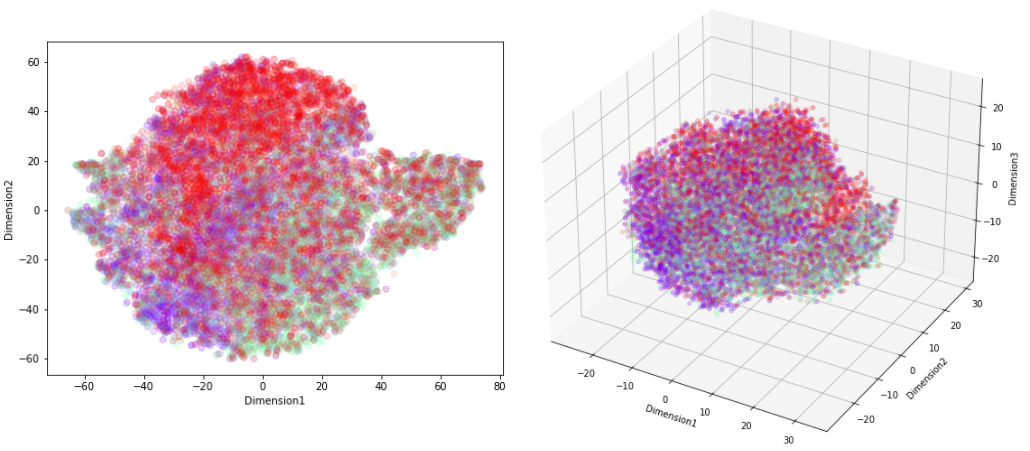
\includegraphics[width=1\columnwidth]{body/figure/figure17.png}
    \captionsetup{labelfont=bf}
    \renewcommand{\baselinestretch}{1.0}
    \caption[Visualization of feature vectors generated by $Inception_{DNA}$]{Visualization of feature vectors generated by $Inception_{DNA}$.}
    \label{f17}
\end{figure}

\begin{figure}[H]
    \centering
    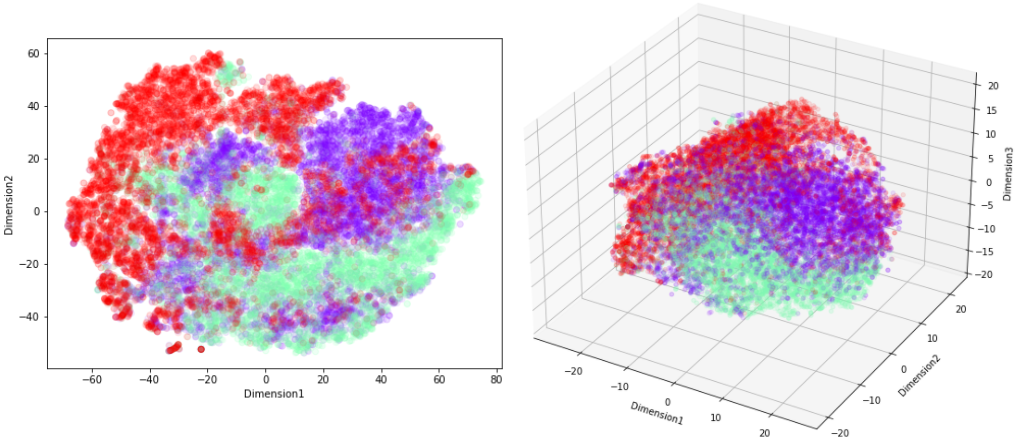
\includegraphics[width=1\columnwidth]{body/figure/figure18.png}
    \captionsetup{labelfont=bf}
    \renewcommand{\baselinestretch}{1.0}
    \caption[Visualization of feature vectors generated by $Inception_{Meth}$]{Visualization of feature vectors generated by $Inception_{Meth}$.}
    \label{f18}
\end{figure}

\begin{figure}[H]
    \centering
    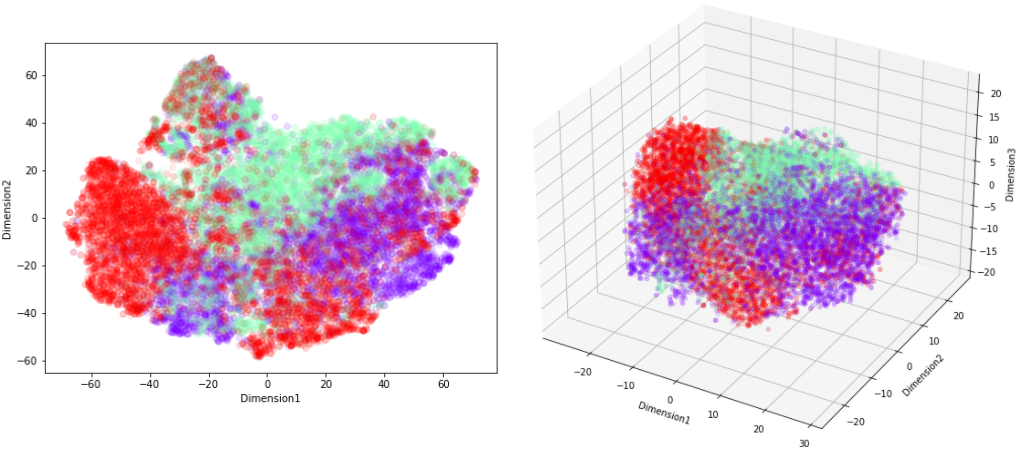
\includegraphics[width=1\columnwidth]{body/figure/figure19.png}
    \captionsetup{labelfont=bf}
    \renewcommand{\baselinestretch}{1.0}
    \caption[Visualization of feature vectors generated by $Inception_{DNA+Meth}$]{Visualization of feature vectors generated by $Inception_{DNA+Meth}$.}
    \label{f19}
\end{figure}

By above visualization, we clearly observe variations of distribution. As long as adding input feature of DNA methylation, the model will learn cell line-specific information via DNA methylation, and automatically discriminate different biosamples within whole feature vectors. This phenomenon is not observed on model only using input features of DNA sequences.

	
\chapter{Conclusions and Future Work} \label{ch:5-conclusion}
	\hspace{24pt}

\section{Conclusions}
In this thesis, we attempt to design a novel CNN framework to predict six core histone modifications from DNA sequences and methylation, for improving data imputation in cell line-specific cases. In our model, we introduce inception module and stratified mini-batch to enhance prediction. By the special architecture of inception module, the use of this module gains better performance than conventional CNN, which is published by DeepSEA. Moreover, in order to handle imbalanced learning, we utilize stratified mini-batch to effectively improve prediction of imbalanced classes, without decrease performance of other classes.

Our model successfully capture useful information from DNA sequences and methylation to predict histone modifications. Shown in our designed experiments, we analyze cases in different combinations of input features. The results show that model integrating features from DNA sequences and methylation outperforms only using features of DNA sequences. Furthermore, we observe that DNA methylation definitely provides cell line-specific insight for model, by visualization.

Therefore, we verify that the DNA methylation strengthens the ability of data imputation for cell line-specific cases, with deep learning model.

\section{Future Work}
According to our study, there are many issues for future researches to explore. We summarize as follow:

\begin{itemize}
\item[$\bullet$] Future studies could increase the number of cell lines to make model extract more overall information from different biosamples.
\item[$\bullet$] Owing to histone is main element of nucleosome, we believe that powerful deep learning model may find out structure of DNA sequences. Therefore, future studies could investigate the association with nucleosome.
\item[$\bullet$] Deep learning field is still growing. Future researches could explore more advanced frameworks whether all of them are good at dealing with this task.
\end{itemize}




%====================
%  Back Pages // cbj
%  1. 參考文獻 2. 附錄 3. 作者簡歷
%====================
%%% 參考文獻
\newpage
\phantomsection % for hyperref to register this
\addcontentsline{toc}{chapter}{References}
\renewcommand{\bibname}{\protect\makebox[5cm][s]{REFERENCES}}
%  \makebox{} is fragile; need protect
\bibliographystyle{unsrt}
%\bibliographystyle{IEEEtranS}  % 使用 IEEE Trans 期刊格式
%  \bibliography{my_bib}

%% References with bibTeX database:
%\bibliographystyle{model1-num-names}
\bibliography{back/ncku_thesis_bibPH}
\baselineskip=18pt
%%\begin{thebibliography}{29}
%%\expandafter\ifx\csname natexlab\endcsname\relax\def\natexlab#1{#1}\fi
%%\providecommand{\bibinfo}[2]{#2}
%%\ifx\xfnm\relax \def\xfnm[#1]{\unskip,\space#1}\fi
%%%Type = Article
%%\bibitem[{Wiegand et~al.(2003)Wiegand, Sullivan, Bjontegaard, and Luthra}]{Wiegand2003}
%%\bibinfo{author}{T.~Wiegand}, \bibinfo{author}{G.~J. Sullivan}, \bibinfo{author}{G.~Bjontegaard}, \bibinfo{author}{A.~Luthra},
%%\newblock \bibinfo{title}{{Overview of the {H.264/AVC} video coding standard}},
%%\newblock \bibinfo{journal}{{\it IEEE Transactions on Circuits and Systems for Video Technology}},
%%\bibinfo{volume}{{\it 13}}(\bibinfo{issue}{7}), \bibinfo{year}{2003}, \bibinfo{pages}{560--576}.
%%%Type = Article
%%\bibitem[{Ostermann et~al.(2004)Ostermann, Bormans, List, Marpe, Narroschke,
%%  Pereira, Stockhammer, and Wedi}]{Ostermann2004}
%%\bibinfo{author}{J.~Ostermann}, \bibinfo{author}{J.~Bormans},
%%  \bibinfo{author}{P.~List}, \bibinfo{author}{D.~Marpe},
%%  \bibinfo{author}{M.~Narroschke}, \bibinfo{author}{F.~Pereira},
%%  \bibinfo{author}{T.~Stockhammer}, \bibinfo{author}{T.~Wedi},
%%\newblock \bibinfo{title}{{Video coding with {H.264/AVC}: tools, performance,
%%  and complexity}},
%%\newblock \bibinfo{journal}{{\it IEEE Circuits and Systems Magazine}},
%%\bibinfo{volume}{{\it 4}}(\bibinfo{issue}{1}), \bibinfo{year}{2004}, \bibinfo{pages}{7--28}.
%%%Type = Article
%%\bibitem[{Marpe et~al.(2006)Marpe, Wiegand, and Sullivan}]{Marpe2006}
%%\bibinfo{author}{D.~Marpe}, \bibinfo{author}{T.~Wiegand},
%%  \bibinfo{author}{G.~J. Sullivan},
%%\newblock \bibinfo{title}{{The {H.264/MPEG4} advanced video coding standard and its applications}},
%%\newblock \bibinfo{journal}{{\it IEEE Communications Magazine}},
%%\bibinfo{volume}{{\it 44}}(\bibinfo{issue}{8}), \bibinfo{year}{2006}, \bibinfo{pages}{134--143}.
%%%Type = Article
%%\bibitem[{Huang et~al.(2005)Huang, Hsieh, Chen, and Chen}]{Huang2005}
%%\bibinfo{author}{Y.-W. Huang}, \bibinfo{author}{B.-Y. Hsieh},
%%\bibinfo{author}{T.-C. Chen}, \bibinfo{author}{L.-G. Chen},
%%\newblock \bibinfo{title}{{Analysis, fast algorithm, and VLSI architecture
%%  design for {H.264/AVC} intra frame coder}},
%%\newblock \bibinfo{journal}{{\it IEEE Transactions on Circuits and Systems for Video Technology}},
%%\bibinfo{volume}{{\it 15}}(\bibinfo{issue}{3}), \bibinfo{year}{2005}, \bibinfo{pages}{378--401}.
%%%Type = Inproceedings
%%\bibitem[{Yu(2004)}]{Yu2004}
%%\bibinfo{author}{A.~C. Yu},
%%\newblock \bibinfo{title}{{Efficient block-size selection algorithm for
%%  inter-frame coding in {H.264/MPEG-4 AVC}}},
%%\newblock \bibinfo{booktitle}{{\it Proc. IEEE Conf. on
%%  Acoustics, Speech, and Signal Processing (ICASSP2004)}}, Montreal, QC, CA, \bibinfo{year}{2004}, \bibinfo{pages}{iii--169--72}.
%%%Type = Article
%%\bibitem[{Wu et~al.(2005)Wu, Pan, Lim, Wu, Li, Lin, Rahardja, and Ko}]{Wu2005}
%%\bibinfo{author}{D.~Wu}, \bibinfo{author}{F.~Pan}, \bibinfo{author}{K.~P. Lim},
%%  \bibinfo{author}{S.~Wu}, \bibinfo{author}{Z.~G. Li},
%%  \bibinfo{author}{X.~Lin}, \bibinfo{author}{S.~Rahardja},
%%  \bibinfo{author}{C.~C. Ko},
%%\newblock \bibinfo{title}{{Fast intermode decision in {H.264/AVC} video
%%  coding}},
%%\newblock \bibinfo{journal}{{\it IEEE Transactions on Circuits and Systems for Video Technology}},
%%  \bibinfo{volume}{{\it 15}}(\bibinfo{issue}{7}), \bibinfo{year}{2005}, \bibinfo{pages}{953--958}.
%%%Type = Article
%%\bibitem[{Grecos and Yang(2006)}]{Grecos2006}
%%\bibinfo{author}{C.~Grecos}, \bibinfo{author}{M.~Yang},
%%\newblock \bibinfo{title}{{Fast mode prediction for the baseline and main
%%  profiles in the {H.264} video coding standard}},
%%\newblock \bibinfo{journal}{{\it IEEE Transactions on Multimedia}},
%%\bibinfo{volume}{{\it 8}}(\bibinfo{issue}{7}), \bibinfo{year}{2006}, \bibinfo{pages}{1125--1134}.
%%%Type = Article
%%\bibitem[{Kannangara et~al.(2006)Kannangara, Richardson, Bystrom, Solera, Zhao, MacLennan, and Cooney}]{Kannangara2006}
%%\bibinfo{author}{C.~S. Kannangara}, \bibinfo{author}{I.~E.~G. Richardson},
%%  \bibinfo{author}{M.~Bystrom}, \bibinfo{author}{J.~R. Solera},
%%  \bibinfo{author}{Y.~Zhao}, \bibinfo{author}{A.~MacLennan},
%%  \bibinfo{author}{R.~Cooney},
%%\newblock \bibinfo{title}{{Low-complexity skip prediction for {H.264} through
%%  Lagrangian cost estimation}},
%%\newblock \bibinfo{journal}{{\it IEEE Transactions on Circuits and Systems for Video Technology}},
%%  \bibinfo{volume}{{\it 16}}(\bibinfo{issue}{2}), \bibinfo{year}{2006}, \bibinfo{pages}{202--208}.
%%%Type = Article
%%\bibitem[{Bharanitharan et~al.(2008)Bharanitharan, Liu, Yang, and
%%  Tsai}]{Bharanitharan2008}
%%\bibinfo{author}{K.~Bharanitharan}, \bibinfo{author}{B.-D. Liu},
%%  \bibinfo{author}{J.-F. Yang}, \bibinfo{author}{W.-C. Tsai},
%%\newblock \bibinfo{title}{{A low complexity detection of discrete cross
%%  differences for fast {H.264/AVC} intra prediction}},
%%\newblock \bibinfo{journal}{{\it IEEE Transactions on Multimedia}},
%% \bibinfo{volume}{{\it 10}}(\bibinfo{issue}{7}), \bibinfo{year}{2008}, \bibinfo{pages}{1250--1260}.
%%%Type = Article
%%\bibitem[{Lee and Lin(2009)}]{Lee2009}
%%\bibinfo{author}{Y.-M. Lee}, \bibinfo{author}{Y.~Lin},
%%\newblock \bibinfo{title}{{Zero-block mode decision algorithm for {H.264/AVC}}},
%%\newblock \bibinfo{journal}{IEEE Transactions on Image Processing},
%%\bibinfo{volume}{{\it 18}}(\bibinfo{issue}{3}), \bibinfo{year}{2009} \bibinfo{pages}{524--533}.
%%%Type = Article
%%\bibitem[{Zeng et~al.(2009)Zeng, Cai, and Ma}]{Zeng2009}
%%\bibinfo{author}{H.~Zeng}, \bibinfo{author}{C.~Cai}, \bibinfo{author}{K.-K.
%%  Ma},
%%\newblock \bibinfo{title}{{Fast mode decision for {H.264/AVC} based on
%%  macroblock motion activity}},
%%\newblock \bibinfo{journal}{{\it IEEE Transactions on Circuits and Systems for Video Technology}},
%%  \bibinfo{volume}{{\it 19}}(\bibinfo{issue}{4}), \bibinfo{year}{2009}, \bibinfo{pages}{491--499}.
%%%Type = Article
%%\bibitem[{Moon et~al.(2005)Moon, Kim, and Kim}]{Moon2005}
%%\bibinfo{author}{Y.~H. Moon}, \bibinfo{author}{G.~Y. Kim},
%%  \bibinfo{author}{J.~H. Kim},
%%\newblock \bibinfo{title}{{An improved early detection algorithm for all-zero
%%  blocks in {H.264} video encoding}},
%%\newblock \bibinfo{journal}{{\it IEEE Transactions on Circuits and Systems for Video Technology}},
%%  \bibinfo{volume}{{\it 15}}(\bibinfo{issue}{8}), \bibinfo{year}{2005}, \bibinfo{pages}{1053--1057}.
%%%Type = Article
%%\bibitem[{Wang et~al.(2006)Wang, Kwong, and Kok}]{Wang2006}
%%\bibinfo{author}{H.~Wang}, \bibinfo{author}{S.~Kwong}, \bibinfo{author}{C.-W. Kok},
%%\newblock \bibinfo{title}{{Efficient prediction algorithm of integer {DCT}
%%  coefficients for {H.264/AVC}optimization}},
%%\newblock \bibinfo{journal}{{\it IEEE Transactions on Circuits and Systems for Video Technology}},
%%  \bibinfo{volume}{{\it 16}}(\bibinfo{issue}{4}), \bibinfo{year}{2006}, \bibinfo{pages}{547--552}.
%%%Type = Article
%%\bibitem[{Wang and Kwong(2007)}]{Wang2007}
%%\bibinfo{author}{H.~Wang}, \bibinfo{author}{S.~Kwong},
%%\newblock \bibinfo{title}{{Hybrid model to detect zero quantized {DCT}
%%  coefficients in {H.264}}},
%%\newblock \bibinfo{journal}{{\it IEEE Transactions on Multimedia}},
%% \bibinfo{volume}{{\it 9}}(\bibinfo{issue}{4}), \bibinfo{year}{2007}, \bibinfo{pages}{728--735}.
%%%Type = Article
%%\bibitem[{Xie et~al.(2007)Xie, Liu, Liu, and Yang}]{Xie2007}
%%\bibinfo{author}{Z.~Xie}, \bibinfo{author}{Y.~Liu}, \bibinfo{author}{J.~Liu},
%%  \bibinfo{author}{T.~Yang},
%%\newblock \bibinfo{title}{{A general method for detecting all-zero blocks prior
%%  to {DCT} and quantization}},
%%\newblock \bibinfo{journal}{{\it IEEE Transactions on Circuits and Systems for Video Technology}},
%%  \bibinfo{volume}{{\it 17}}(\bibinfo{issue}{2}), \bibinfo{year}{2007}, \bibinfo{pages}{237--241}.
%%%Type = Article
%%\bibitem[{Sousa(2000)}]{Sousa2000}
%%\bibinfo{author}{L.~A. Sousa},
%%\newblock \bibinfo{title}{{General method for eliminating redundant computations in video coding}},
%%\newblock \bibinfo{journal}{{\it Electronics Letters}},
%%\bibinfo{volume}{36}(\bibinfo{issue}{2}), \bibinfo{year}{2000}, \bibinfo{pages}{306--307}.
%%%Type = Article
%%\bibitem[{Pao and Sun(1999)}]{Pao1999}
%%\bibinfo{author}{I.-M. Pao}, \bibinfo{author}{M.-T. Sun},
%%\newblock \bibinfo{title}{{Modeling {DCT} coefficients for fast video
%%  encoding}},
%%\newblock \bibinfo{journal}{{\it IEEE Transactions on Circuits and Systems for Video Technology}},
%%  \bibinfo{volume}{{\it 9}}(\bibinfo{issue}{4}),\bibinfo{year}{1999},\bibinfo{pages}{608--616}.
%%%Type = Manual
%%\bibitem[{Sta(2007)}]{StandardAVC}
%%\bibinfo{title}{{{ITU}-T Recommendation H.264 : Advanced video coding for
%%  generic audiovisual services}}, \bibinfo{organization}{International
%%  Telecommunications Union}, \bibinfo{year}{2007}.
%%%Type = Book
%%\bibitem[{Richardson(2003)}]{Richardson2003}
%%\bibinfo{author}{I.~Richardson}, \bibinfo{title}{{\it H.264 and MPEG-4 video
%%  compression: video coding for next-generation multimedia}},
%%  (\bibinfo{publisher}{Wiley}, \bibinfo{year}{2003}).
%%%Type = Article
%%\bibitem[{Lam and Goodman(2000)}]{Lam2000}
%%\bibinfo{author}{E.~Y. Lam}, \bibinfo{author}{J.~W. Goodman},
%%\newblock \bibinfo{title}{{A mathematical analysis of the DCT coefficient
%%  distributions for images}},
%%\newblock \bibinfo{journal}{{\it IEEE Transactions on Image Processing}},
%% \bibinfo{volume}{{\it 9}}(\bibinfo{issue}{10}), \bibinfo{year}{2000}, \bibinfo{pages}{1661--1666}.
%%%Type = Article
%%\bibitem[{Reininger(1983)}]{Reininger1983}
%%\bibinfo{author}{R.~Reininger} \& \bibinfo{author}{J.~Gibson},
%%\newblock \bibinfo{title}{{Distribution of the two dimensional dct coefficients
%%  for images}},
%%\newblock \bibinfo{journal}{{\it IEEE Transactions on Communications}},
%% \bibinfo{volume}{{\it 31}}(\bibinfo{issue}{6}), \bibinfo{year}{1983}, \bibinfo{pages}{835--839}.
%%%Type = Inproceedings
%%\bibitem[{Altunbasak and Kamaci(2004)}]{Altunbasak2004}
%%\bibinfo{author}{Y.~Altunbasak}, \bibinfo{author}{N.~Kamaci},
%%\newblock \bibinfo{title}{{An analysis of the DCT coefficient distribution with
%%  the H.264 video coder}},
%%\newblock \bibinfo{booktitle}{{\it Proc. IEEE Conf. on Acoustics, Speech, and Signal Processing (ICASSP2004)}}, Montreal, QC, CA, \bibinfo{year}{2004},
%%\bibinfo{pages}{iii --177--80}.
%%%Type = Book
%%\bibitem[{Eude et~al.(1994{\natexlab{a}})Eude, Cherifi, and Grisel}]{Eude1994a}
%%\bibinfo{author}{T.~Eude}, \bibinfo{author}{H.~Cherifi},
%%  \bibinfo{author}{R.~Grisel}, \bibinfo{title}{{Statistical distribution of DCT
%%  coefficients and their application to an adaptive compression algorithm}},
%%  \newblock \bibinfo{booktitle}{{\it IEEE Region 10 Conf. (TENCON1994)}}, \bibinfo{year}{1994}, Singapore, Singapore, \bibinfo{pages}{427--430}.
%%%Type = Inproceedings
%%\bibitem[{Eude et~al.(1994{\natexlab{b}})Eude, Grisel, Cherifi, and
%%  Debrie}]{Eude1994b}
%%\bibinfo{author}{T.~Eude}, \bibinfo{author}{R.~Grisel},
%%  \bibinfo{author}{H.~Cherifi}, \bibinfo{author}{R.~Debrie},
%%\newblock \bibinfo{title}{{On the distribution of the DCT coefficients}},
%%\newblock \bibinfo{booktitle}{{\it Proc. IEEE Conf. on Acoustics, Speech, and Signal Processing (ICASSP1994)}},
%%  \bibinfo{year}{1994}, Adelaide, SA, AU, \bibinfo{pages}{v--365--368}.
%%%Type = Article
%%\bibitem[{Xie and Chia(2008)}]{Xie2008}
%%\bibinfo{author}{J.~Xie}, \bibinfo{author}{L.-T. Chia},
%%\newblock \bibinfo{title}{{\it Study on the distribution of DCT residues and its
%%  application to R-D analysis of video coding}},
%%\newblock \bibinfo{journal}{Journal of Visual Communication and Image Representation},
%% \bibinfo{volume}{19}(\bibinfo{issue}{7}), \bibinfo{year}{2008}, \bibinfo{pages}{411--425}.
%%%Type = Book
%%\bibitem[{Jain(1989)}]{Jain1989}
%%\bibinfo{author}{A.~Jain}, \bibinfo{title}{{\it Fundamentals of digital image
%%  processing}} (\bibinfo{publisher}{Inc. Upper Saddle River, NJ:Prentice-Hall}, \bibinfo{year}{1989}).
%%%Type = Article
%%\bibitem[{Hang and Chen(1997)}]{Hang1997}
%%\bibinfo{author}{H.-M. Hang}, \bibinfo{author}{J.-J. Chen},
%%\newblock \bibinfo{title}{{Source model for transform video coder and its
%%  application - Part I: Fundamental theory}},
%%\newblock \bibinfo{journal}{{\it IEEE Transactions on Circuits and Systems for Video Technology}},
%% \bibinfo{volume}{{\it 7}}(\bibinfo{issue}{2}), \bibinfo{year}{1997}, \bibinfo{pages}{287--298}.
%%%Type = Article
%%\bibitem[{Ma(2005)}]{Ma2005}
%%\bibinfo{author}{S.~Ma},
%%\newblock \bibinfo{title}{{Rate-distortion analysis for H.264/AVC video coding
%%  and its application to rate control}},
%%\newblock \bibinfo{journal}{{\it IEEE Transactions on Circuits and Systems for Video Technology}},
%% \bibinfo{volume}{{\it 15}}(\bibinfo{issue}{12}), \bibinfo{year}{2005}, \bibinfo{pages}{1533--1544}.
%%%Type = Manual
%%\bibitem[{JMS(2008)}]{JMSoftware}
%%\bibinfo{title}{{{H.264/AVC} reference software, Joint Model (JM), [{O}nline]. Available:
%%  http://iphome.hhi.de/suehring/tml/}}.

%%\end{thebibliography}


%%% 附錄
%%
% this file is encoded in utf-8
% v2.0 (Apr. 5, 2009)
%%% 每一個附錄 (附錄甲、附錄乙、...) 都要複製此段附錄編排碼做為起頭
%%% 附錄編排碼 begin >>>
\newpage
\chapter*{Appendix A: MATLAB / Octave } % 修改附錄編號與你的附錄名
\phantomsection % for hyperref to register this
\addcontentsline{toc}{chapter}{Appendix A: MATLAB / Octave} %建議此內容應與上行相同
%\setcounter{chapter}{0}  %如果用的是 TeXLive2007 則打開此行以避免錯誤
\setcounter{equation}{0} 
\setcounter{figure}{0} 
\setcounter{footnote}{0} 
\setcounter{section}{0} 
\setcounter{subsection}{0}
\setcounter{subsubsection}{0}
\setcounter{table}{0} 
\renewcommand{\thechapter}{A} % 如果是附錄乙,則內容應為{乙}
%%% <<< 附錄編排碼 end

% 附錄內容開始
% 納入程式源碼
%\lstinputlisting{example_prog_list.m}


\begin{equation}\sum_{k=1}^{n} k = \frac{n(n+1)}{2}\end{equation}

%%% 如果有附錄乙、丙、...,則在此繼續加上「附錄編排」碼
% 每一個附錄會自動以新頁開始
%%% 自傳
%\newpage
\chapter*{\nameVita} % \makebox{} is fragile; need protect
\phantomsection % for hyperref to register this
\addcontentsline{toc}{chapter}{\nameVitac}

\noindent
{\it Bo-Jhih Chen} received his B.S. and M.S. degree in I-Shou University, Kaohsiung, Taiwan (R.O.C.), in 2004 and 2006, respectively. He got his Ph.D. degree of the Institute of Computer and Communication Engineering at Department of Electrical Engineering in National Cheng Kung University, Tainan, Taiwan (R.O.C.), in 2012.
His research interests are in the areas of video coding standards, digital signal processing, and multimedia system.
\bigskip \\
\noindent {\bf Education Background}\\
\noindent Sept. 2006 -- June 2012:\\
	Ph.D., Institute of Computer and Communication Engineering, Department of Electrical Engineering, National Cheng Kung University.\\
\noindent Sept. 2004 -- June 2006:\\
	M.S., Department of Computer Science and Information Engineering, I-Shou University.\\
\noindent Sept. 2000 -- June 2004:\\
	B.S., Department of Computer Science and Information Engineering, I-Shou University.

\clearpage % to make sure all CJK characters are processed
\end{CJK}  %%% ZZZ %%%
\end{document}

